\chapter{基準系、光、そして時空の幾何学}

\section{相対性理論から再び始まる講義}

今学期は古典物理学に戻るが、空間と時間が独立で普遍的であるニュートン的描像に戻るのではない。当面の主題は特殊相対性理論と古典場の理論、とりわけ電磁気学である。量子力学は用いない。以前の力学の講義では作用原理ならびにハミルトニアンおよびラグランジアンによる記述が与えられ、量子力学の講義ではその基本原理が与えられたが、調和振動子さえも後の回帰に委ねざるを得なかった。光もまたほとんど扱われなかった。その欠落は今ここで埋められる。光は本質的に相対論的だからである。

このクラスの大半は特殊相対性理論に以前出会ったことがある。それでも挙手によって、それを初めから再構築することが支持された。それが有用な選択である。ローレンツ変換は暗記すべき公式として導入されるべきではない。それは、空間と時間の操作的測定がガリレイ的運動学と観測された光の伝播法則の双方を同時に満たしえないことから、自然に現れるべきものである。

\subsection{物理的装置としての座標}

デカルト系から始める。すなわち原点、三つの向き付けられた軸、そして座標\(x,y,z\)である。具体的な実現としては、空間を剛体のメートル尺の点陣で満たせばよい。単なる場所ではなく事象を同定するために、点陣の各点は時計も備える。すると事象は
\begin{equation}
(x,y,z,t).
\end{equation}
とラベル付けされる。時計は何らかの明示された手続きによって同期されねばならない。その要請はまもなくこの構成の微妙な部分となる。

\begin{definition}
基準系とは、空間座標の点陣と、分散配置された同期時計の系とを合わせたものである。慣性系とは、回転も加速もしない系であって、そこでは力を受けないすべての粒子が一定の速度で運動する。
\end{definition}

相対的な一様運動にある二つの系は、同じ事象に異なる座標を割り当てる。運動系に固定された点は、そのプライムなし座標が変化している間も、一定の座標\(x'\)をもつ。\(x\)方向に沿った運動について、ニュートン物理学における空間的関係は
\begin{equation}
x'=x-vt.
\label{eq:sr1-galilean-space}
\end{equation}
である。より目立たないニュートンの仮定は、正しく合わせられたすべての腕時計が普遍的に同期したままだというものである。
\begin{equation}
t'=t.
\label{eq:sr1-absolute-time}
\end{equation}

\subsection{相対性原理}

相対性理論はアインシュタインから始まったのではない。ガリレオとニュートンはすでに、物理法則がすべての慣性系で同じ形をとるという原理を用いていた。ニュートンの法則\(F=ma\)、重力の逆二乗則、そしてクーロン力は、実験室が一様に運動するというだけでは新たな形を獲得しない。

よく知られた検証は密閉された鉄道車両である。列車が滑らかに動き、窓が外の何も見せないなら、ジャグリングは静止した部屋での場合とまったく同じに振る舞う。ボールは通常どおりに上がり、落ち、手に戻る。車両内に閉じ込められた実験はその一様な速度を明らかにできない。加速度や回転は内部で検出できるが、一様な並進運動は検出できない。

アインシュタインはこの古い原理に一つの物理法則を加える。真空中の光は
\begin{equation}
c \simeq 1.86\times 10^5\ {\rm miles/s}
   \simeq 3.00\times 10^8\ {\rm m/s}.
\end{equation}
で伝播する。これが自然の法則であり、法則がすべての慣性系で同じであるなら、すべての慣性観測者は同じ\(c\)を測定しなければならない。

\section{なぜガリレイ変換は失敗するのか}

この衝突を露呈させるには一次元の空間で十分である。横軸を\(x\)、縦軸を\(t\)とする時空図を描く。原点から放出され右へ進む光パルスは
\begin{equation}
x=ct.
\label{eq:sr1-light-right}
\end{equation}
に従う。速度\(v\)で右へ運動する系の原点は
\begin{equation}
x=vt,
\qquad
x'=0.
\label{eq:sr1-moving-origin}
\end{equation}
の上にある。

\begin{figure}[htbp]
\centering
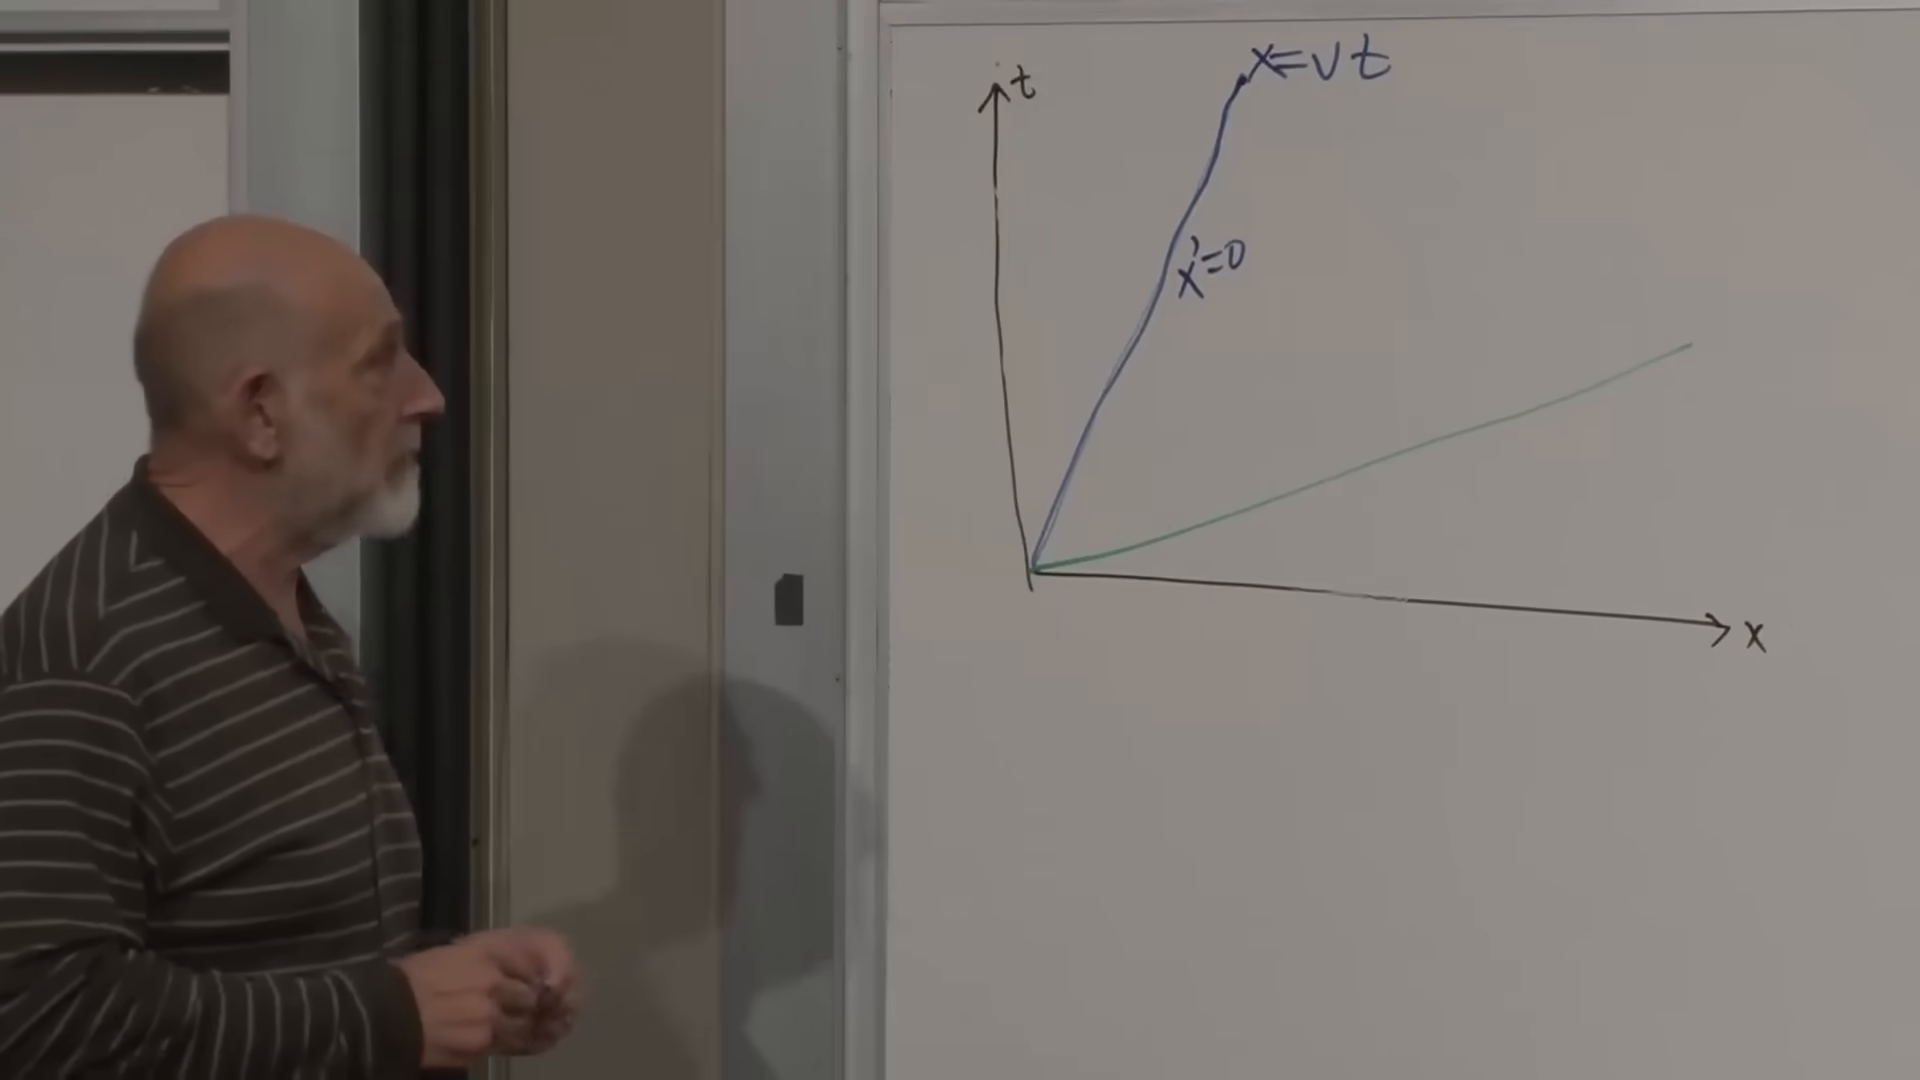
\includegraphics[width=0.90\textwidth]{lecture_01_figure_01.png}
\caption{右へ進む光線と、運動する原点\(x=vt\)。プライム付き観測者はこれを\(x'=0\)とラベル付けする。}
\lectureframe{00:15:24}
\end{figure}

ガリレイの規則\eqref{eq:sr1-galilean-space}--\eqref{eq:sr1-absolute-time}を光線に適用すると、
\begin{align}
x'&=x-vt=(c-v)t,\\
t'&=t.
\end{align}
となる。したがってプライム付き観測者は
\begin{equation}
x'=(c-v)t',
\end{equation}
と推論するであろうから、右へ進む光の速さは\(c-v\)となる。左へ進む光線\(x=-ct\)については、
\begin{equation}
x'=-(c+v)t',
\end{equation}
であり、その速さの大きさは\(c+v\)である。

\begin{figure}[htbp]
\centering
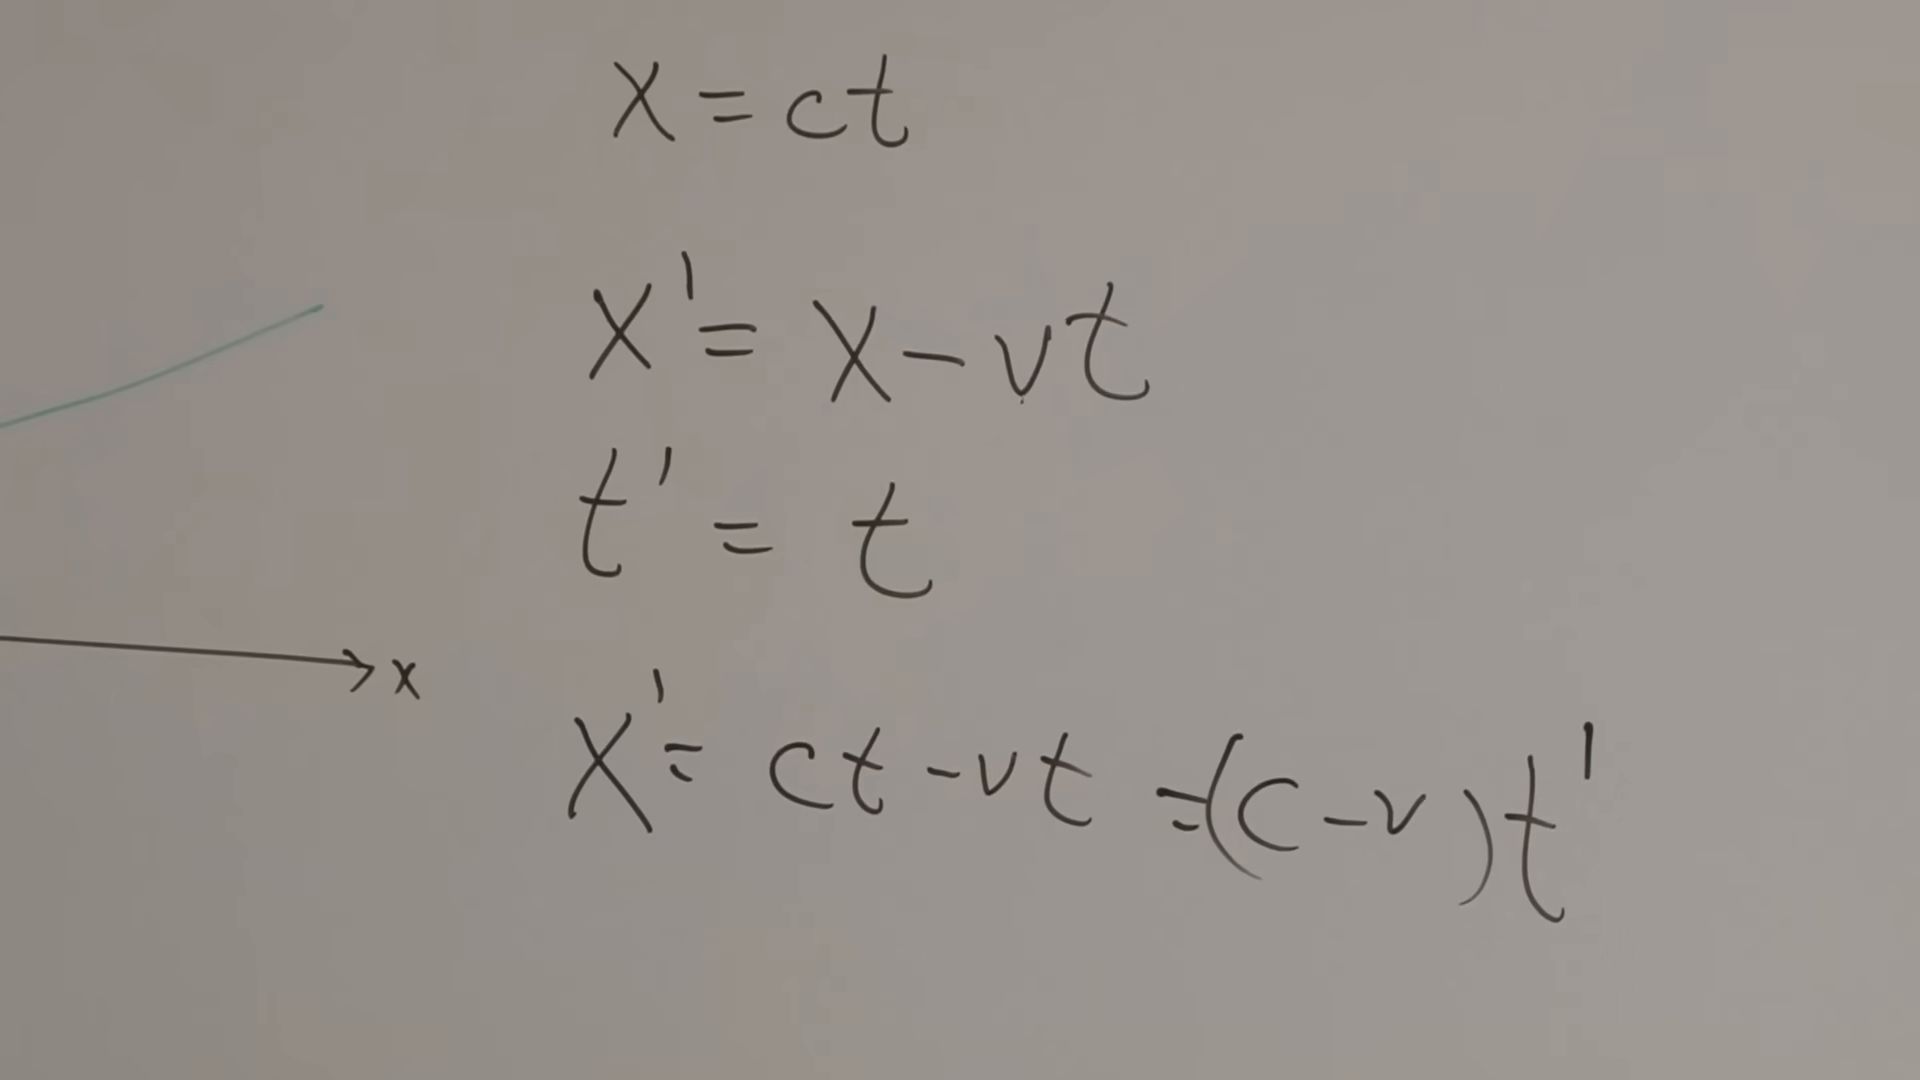
\includegraphics[width=0.90\textwidth]{lecture_01_figure_02.png}
\caption{ガリレイ的置き換えは右へ進む光線に対して\(c-v\)を予測し、系に依存しない光速と矛盾する。}
\lectureframe{00:17:23}
\end{figure}

通常の速度の合成は遅い力学的運動に対しては優れた近似であるが、光の測定は予測される\(c-v\)や\(c+v\)を示さない。再考されるべきは光の要請ではなく変換法則である。中心的な容疑者は、一見無害な命題\(t'=t\)である。それは同時性の絶対的な概念を主張している。

\section{遠方の時計の同期}

異なる場所にある二つの時計が同じ時刻を示すと言うには、実験が必要である。それらの中点に第三の観測者を置き、等しい距離は物差しによって確定する。両端の時計に、それぞれが正午を指したときに閃光を発するよう指示する。その閃光が同時に中点へ到達すれば、それらの時計は同期していると呼ぶ。

これは物理学の上にかぶせられた哲学的定義ではない。時計と距離と光信号から作られた再現可能な操作である。

次に、ある観測者が中点のそばを通過して運動するとしよう。静止した中点に同時に到着する両端からの閃光は、運動する観測者には同時には到着しない。光が飛んでいる間に、その観測者は一方の閃光へ近づき、他方から遠ざかるからである。したがって、静止した時計によって同時と判定された事象は、運動する系の同様に妥当な同期手順によれば同時ではない。

プライムなしの系において、同時事象の線は
\begin{equation}
t=\text{constant}.
\end{equation}
である。対応するプライム付きの線は、\(x\)-\(t\) 図において傾くであろう。変換公式を求める前に、光信号を用いてその傾きを構成することができる。

\section{光で描かれた運動系}

\(c=1\) とせよ。時間を秒で測るときには距離を光秒で測ってもよく、あるいは選んだ長さの単位一つを横切る光の走行時間によって時間を測ってもよい。どちらの規約でも、光線は
\begin{equation}
x=\pm t,
\label{eq:sr1-light-units}
\end{equation}
となり、したがって等しい目盛りの軸上で \(45^\circ\) の線となる。

まず光線を描く。次に、運動系で静止している観測者の族を描く：
\begin{equation}
x=vt,\qquad x=vt+1,\qquad x=vt+2.
\label{eq:sr1-moving-family}
\end{equation}
それらの世界線は平行である。観測者たちは自分たちの慣性格子において固定した間隔を保つからである。

\begin{figure}[htbp]
\centering
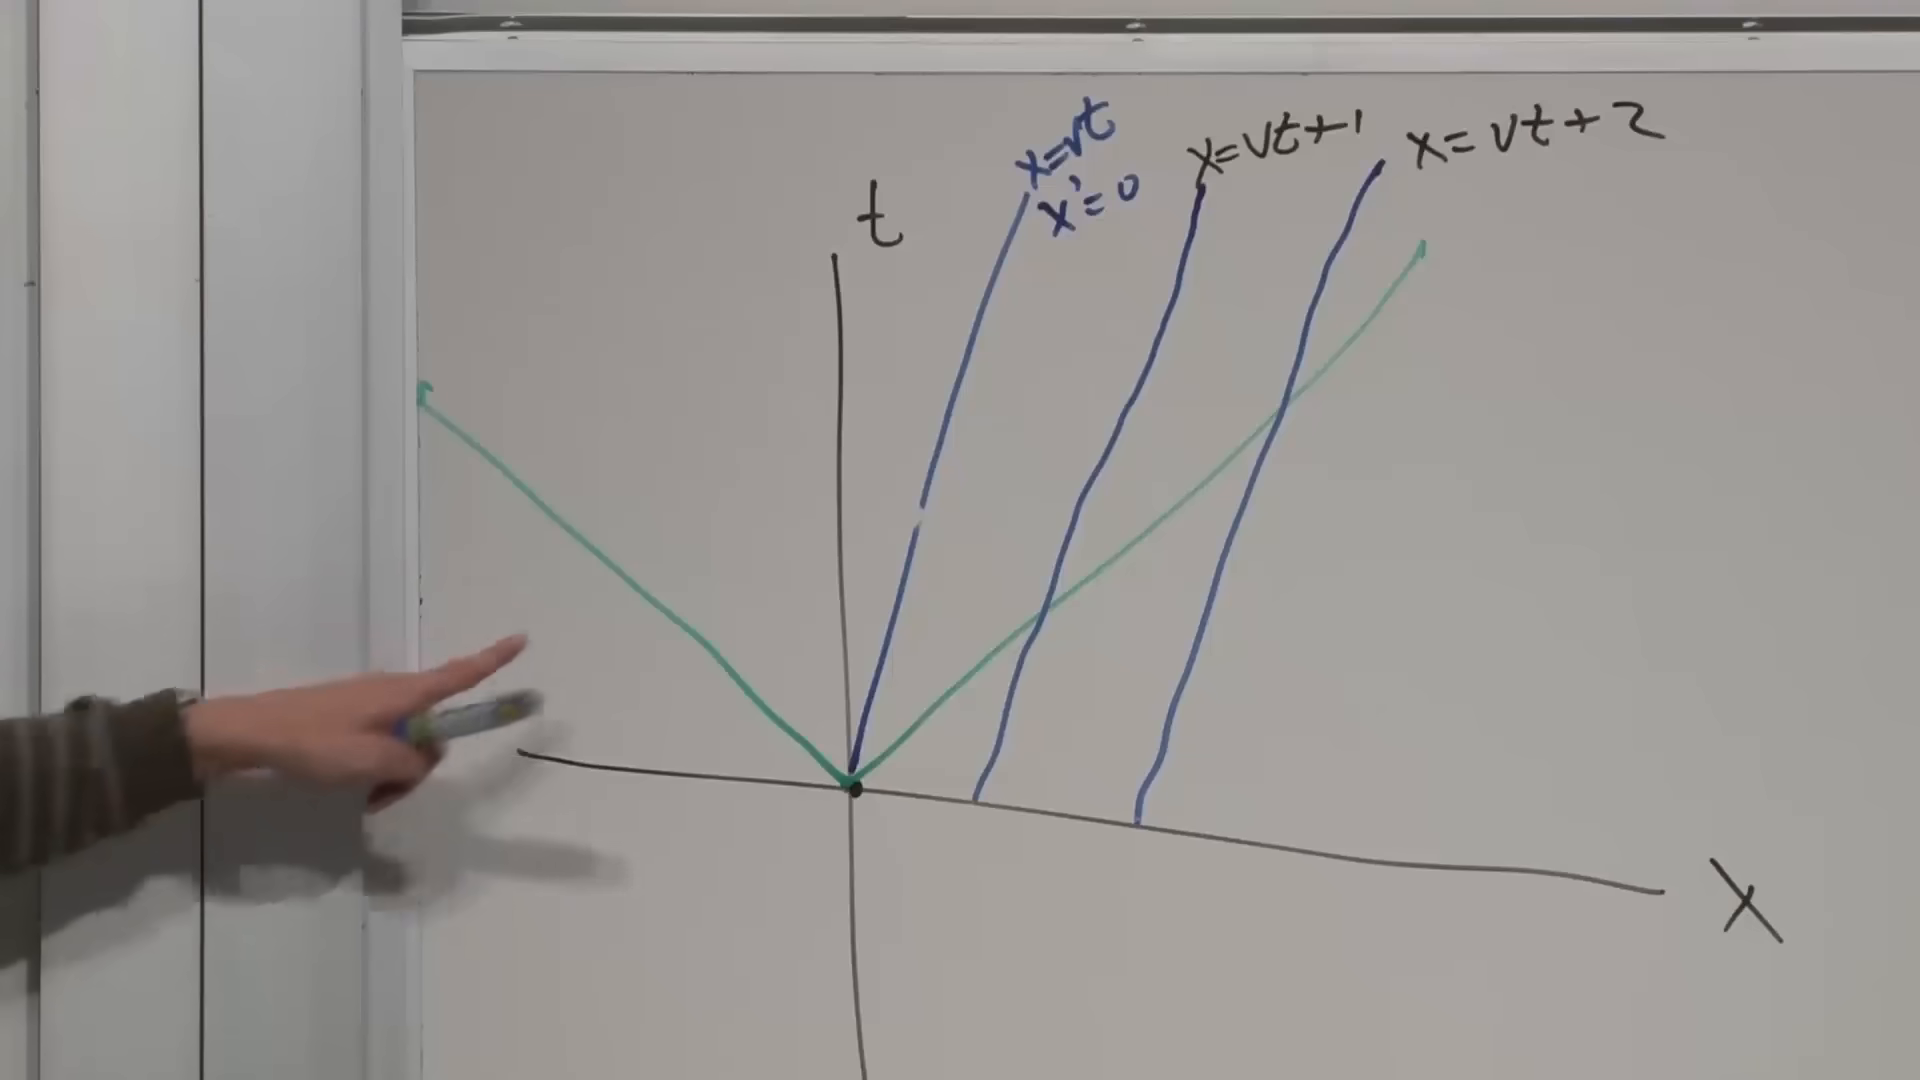
\includegraphics[width=0.90\textwidth]{lecture_01_figure_03.png}
\caption{\(45^\circ\) における光線と、運動する座標格子の平行な世界線 \(x=vt\)、\(x=vt+1\)、\(x=vt+2\)。}
\lectureframe{00:29:55}
\end{figure}

\subsection{フレッド、メアリー、シーモア}

フレッドが \(x=vt\) を占め、メアリーが \(x=vt+1\) を占め、シーモアが \(x=vt+2\) を占めるとする。原点 \(O\) において、フレッドは右向きの光信号をメアリーへ送る。シーモアは左向きの信号を送り、二つの閃光が同じ事象 \(a\) でメアリーに到達するようにする。運動系の中点同期規則により、シーモアの発射事象 \(b\) はフレッドの \(O\) における発射と同時である。したがって \(O\) と \(b\) を通る線は \(t'=0\) である。

事象 \(a\) は
\begin{equation}
x=t
\end{equation}
と
\begin{equation}
x=vt+1.
\end{equation}
の両方の上にある。したがって、
\begin{equation}
t_a=x_a=\frac{1}{1-v}.
\label{eq:sr1-event-a}
\end{equation}

\(a\) を通る左向きの光線は
\begin{equation}
x+t=x_a+t_a=\frac{2}{1-v}.
\label{eq:sr1-ab-light}
\end{equation}
を満たす。事象 \(b\) はシーモアの世界線上にもあり、
\begin{equation}
x-vt=2.
\label{eq:sr1-seymour-line}
\end{equation}
\eqref{eq:sr1-ab-light} と \eqref{eq:sr1-seymour-line} を解くと
\begin{align}
t_b&=\frac{2v}{1-v^2},\\
x_b&=\frac{2}{1-v^2}.
\label{eq:sr1-event-b}
\end{align}
したがって \(O\) から \(b\) への線の傾きは
\begin{equation}
\frac{t_b}{x_b}=v,
\end{equation}
となり、運動する同時線は
\begin{equation}
t=vx,
\qquad
t'=0.
\label{eq:sr1-moving-simultaneity}
\end{equation}
である。

\begin{figure}[htbp]
\centering
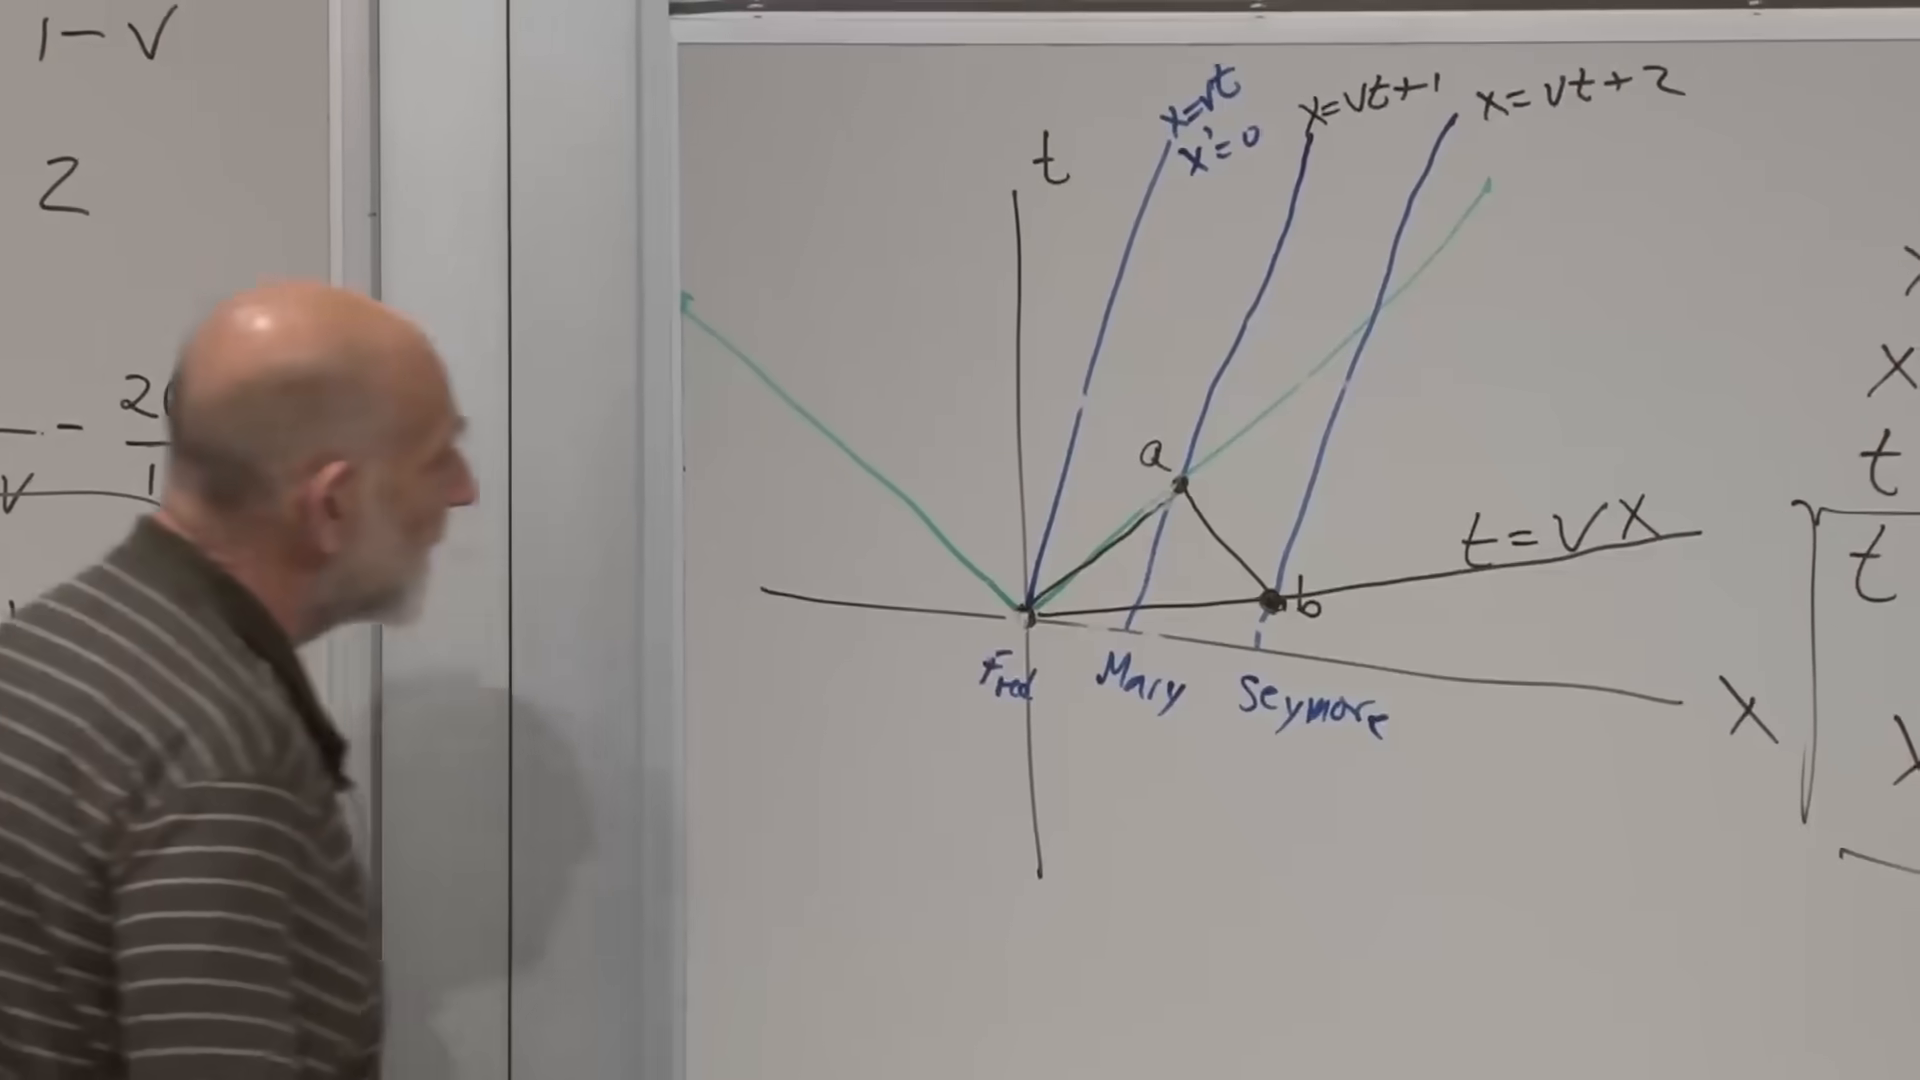
\includegraphics[width=0.93\textwidth]{lecture_01_figure_04.png}
\caption{フレッド--メアリー--シーモアの同期構成。同時に到着する光信号が、運動系において \(O\) と \(b\) を同時と同定し、\(t=vx\) を与える。}
\lectureframe{00:44:38}
\end{figure}

プライム付きの系の二つの軸は今や平行な形をとる：
\begin{align}
x'=0 &\quad\Longleftrightarrow\quad x=vt,\\
t'=0 &\quad\Longleftrightarrow\quad t=vx.
\end{align}
それらは右向きの光線 \(x=t\) に関して互いに鏡映である。この幾何学はすでに普遍的な同時性を置き換えている。

\begin{classroomqa}
\audiencequestion{\(v=1\) または \(v=-1\) のとき、この構成はどうなるか。}
\lecturerresponse{\eqref{eq:sr1-event-a}--\eqref{eq:sr1-event-b} の分母が消え、関連する交点は無限遠へ退く。\(\lvert v\rvert=1\) では、物質的な観測者は光線上を運動することになり、通常の中点交換を完了できない。この特異な振る舞いは、\(c\) が限界速度であるという最初の幾何学的警告である。\lecturetimestamp{00:40:43}}
\end{classroomqa}

\section{ローレンツ変換の導出}

\(x=vt\) 上の \(x'=0\) という条件は、\(x'\) が因子 \(x-vt\) を含むことを要求する。同様に、\(t=vx\) 上の \(t'=0\) は因子 \(t-vx\) を要求する。時空の一様性により変換は線形となるので、
\begin{align}
x'&=(x-vt)f(v),\\
t'&=(t-vx)g(v).
\label{eq:sr1-linear-ansatz}
\end{align}
と書く。

\begin{figure}[htbp]
\centering
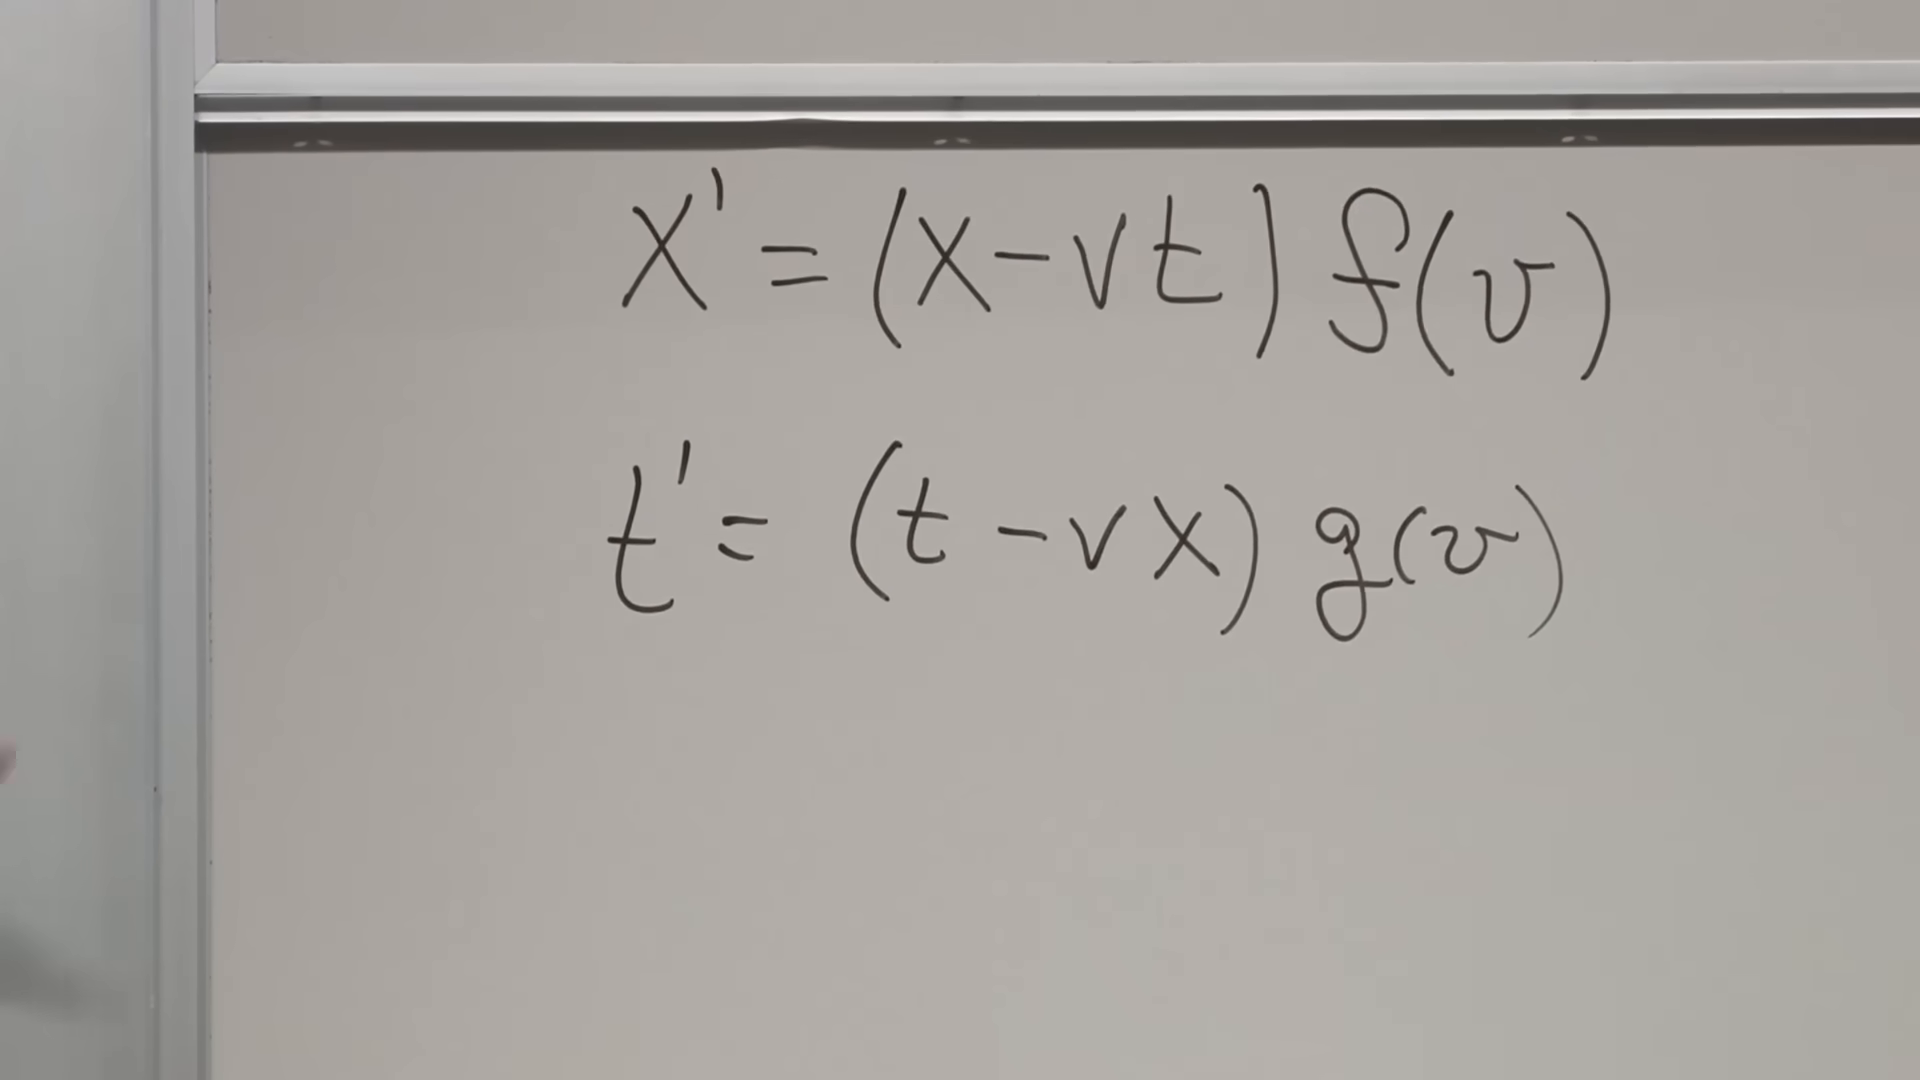
\includegraphics[width=0.90\textwidth]{lecture_01_figure_05.png}
\caption{この線形変換は二つの消滅条件から組み立てられ、速度に依存する尺度因子 \(f(v)\) と \(g(v)\) をもつ。}
\lectureframe{00:49:35}
\end{figure}

右向きの光線 \(x=t\) に沿って、光速度の不変性は \(x'=t'\) を要求する。そのとき式~\eqref{eq:sr1-linear-ansatz}は
\begin{align}
x'&=(1-v)x f(v),\\
t'&=(1-v)x g(v),
\end{align}
となり、したがって
\begin{equation}
f(v)=g(v).
\label{eq:sr1-f-equals-g}
\end{equation}
となる。こうして一つの共通の尺度因子が残る：
\begin{align}
x'&=(x-vt)f(v),\\
t'&=(t-vx)f(v).
\label{eq:sr1-direct-unscaled}
\end{align}
これは本質的に、アインシュタインの最初の相対性理論論文で用いられた簡潔な論証の道筋である。操作的な同時性と不変な光速度が変換を決定する。

\subsection{相互性が尺度を定める}

特別な\emph{本当に運動している}慣性系というものは存在しない。プライム付きの系がプライムなしの系に対して\(v\)で運動しているなら、プライムなしの系はプライム付きの系に対して\(-v\)で運動している。したがって、逆写像も\(v\)の符号を反転させた同じ形でなければならない：
\begin{align}
x&=(x'+vt')f(v),\\
t&=(t'+vx')f(v).
\label{eq:sr1-inverse-unscaled}
\end{align}

\begin{figure}[htbp]
\centering
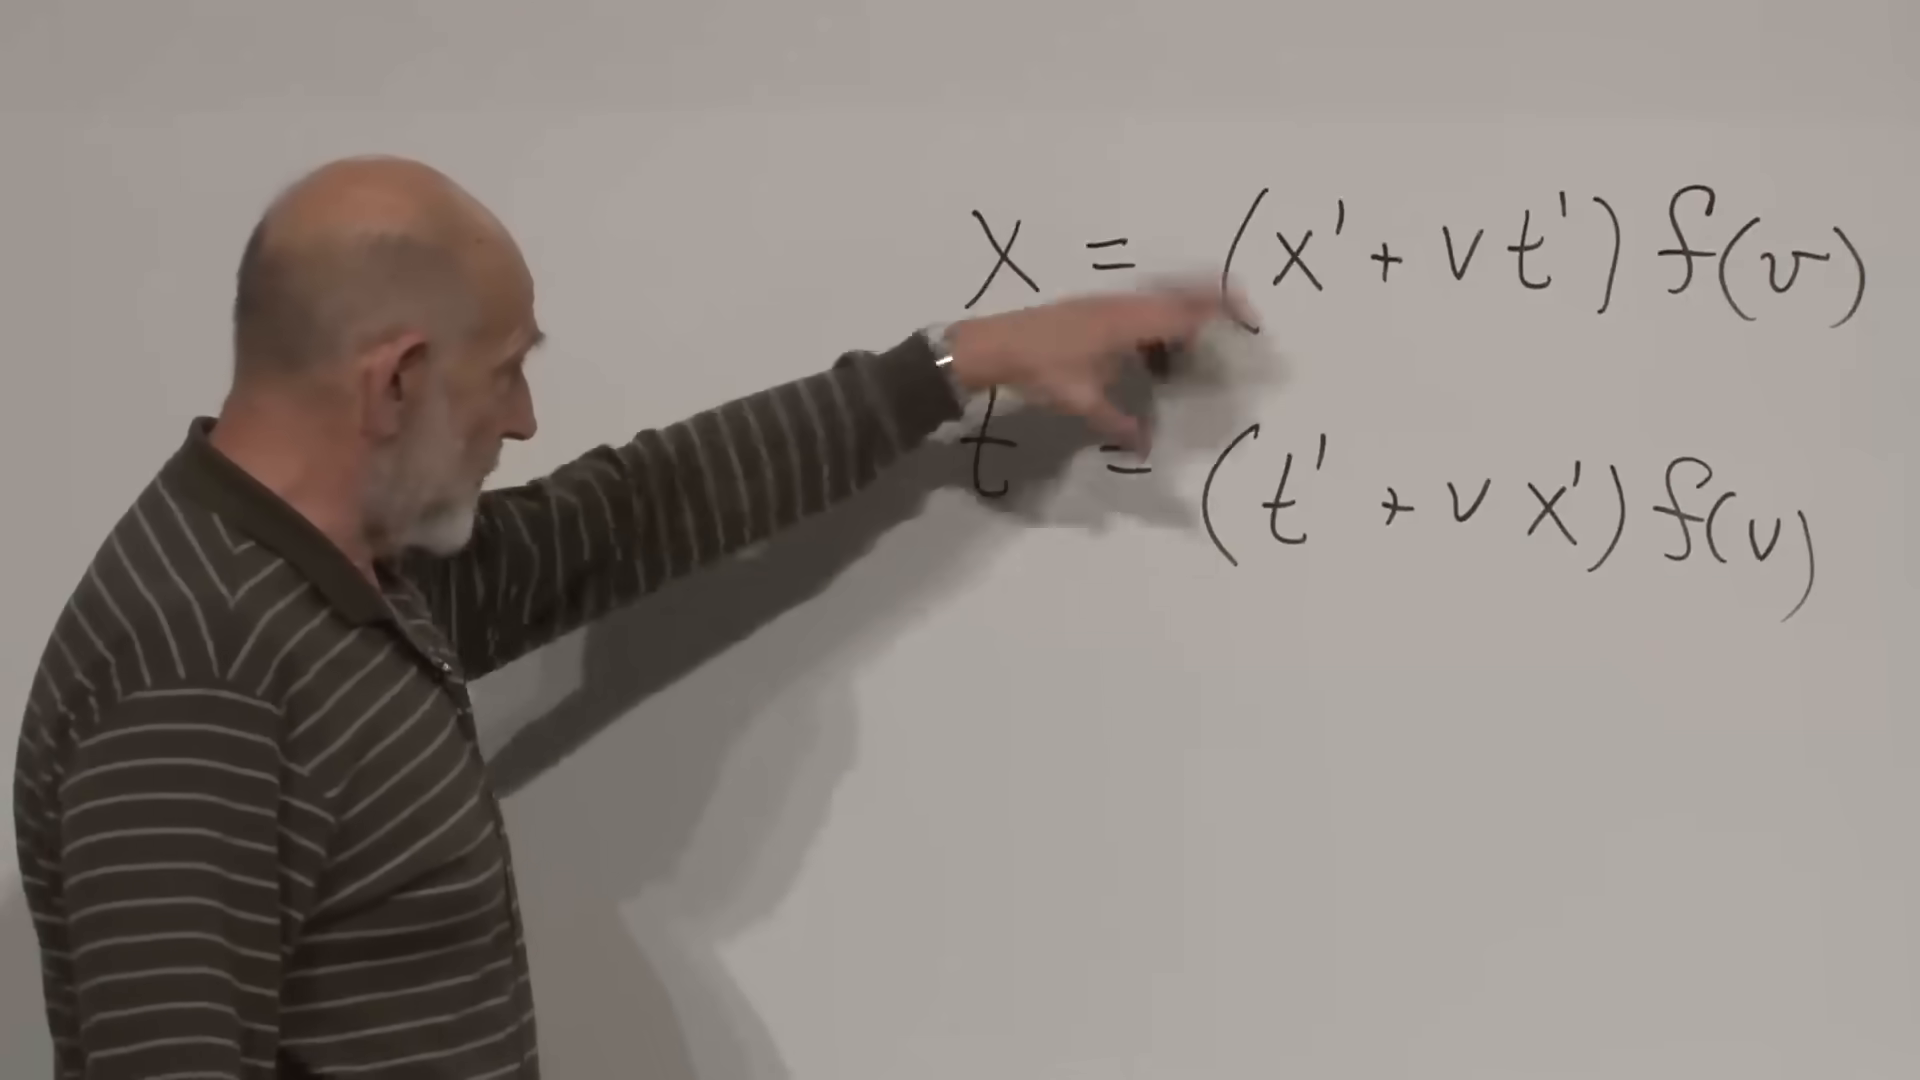
\includegraphics[width=0.90\textwidth]{lecture_01_figure_06.png}
\caption{相反性により、逆変換は相対速度を反転させ、同じスケール因子を保つことで得られる。}
\lectureframe{00:55:12}
\end{figure}

\eqref{eq:sr1-direct-unscaled}を\eqref{eq:sr1-inverse-unscaled}の第一式に代入すると：
\begin{align}
x
&=\left[(x-vt)f(v)+v(t-vx)f(v)\right]f(v)\\
&=x(1-v^2)f(v)^2.
\end{align}
この合成が恒等写像でなければならないので、
\begin{equation}
(1-v^2)f(v)^2=1,
\end{equation}
したがって
\begin{equation}
f(v)=\pm\frac{1}{\sqrt{1-v^2}}.
\label{eq:sr1-factor-roots}
\end{equation}

\begin{figure}[htbp]
\centering
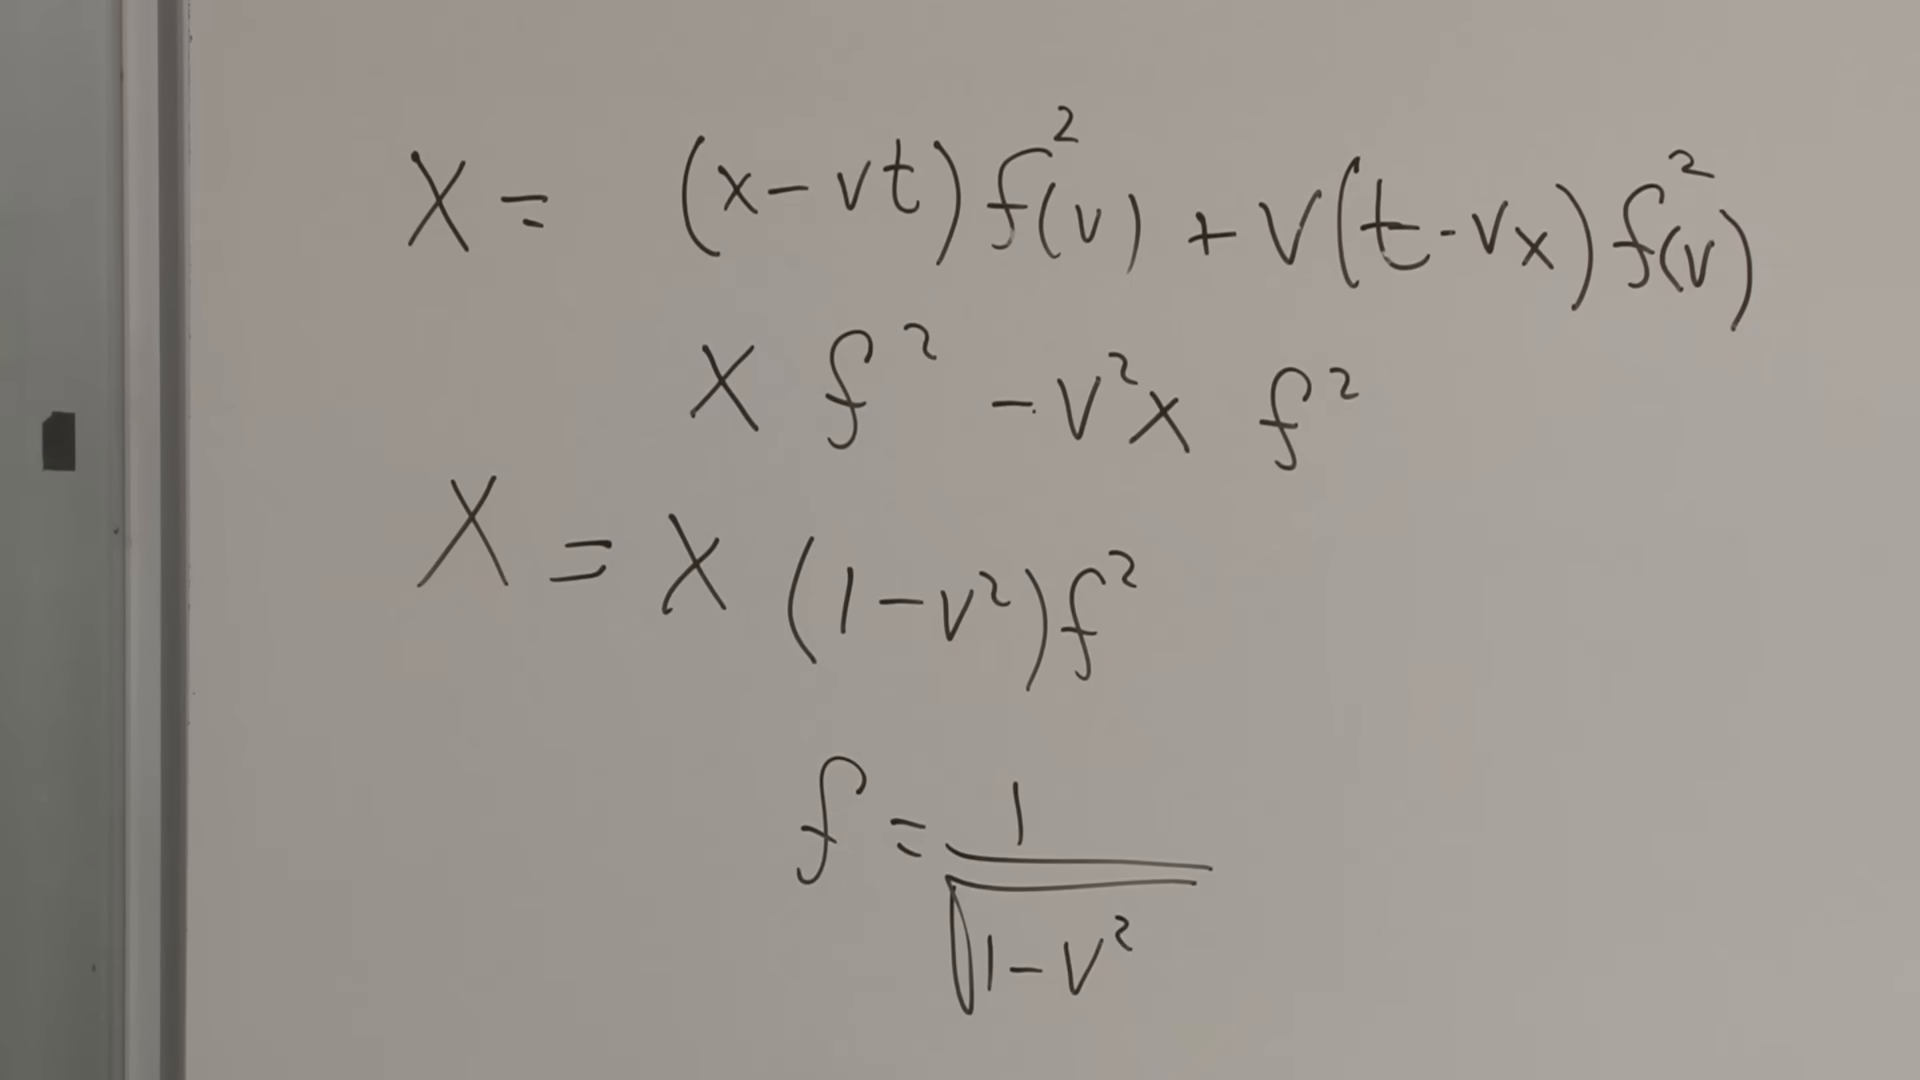
\includegraphics[width=0.90\textwidth]{lecture_01_figure_07.png}
\caption{直接写像と逆写像を合成すると、共通因子\(f(v)\)の大きさが定まる。}
\lectureframe{00:59:31}
\end{figure}

\begin{classroomqa}
\audiencequestion{なぜ\eqref{eq:sr1-factor-roots}における負の平方根を捨てるのか？}
\lecturerresponse{相対速度がゼロのとき、変換は連続的に恒等変換に近づかなければならず、\(x'=x\)かつ\(t'=t\)である。負の分枝は代わりに\(x'=-x\)かつ\(t'=-t\)を与え、両方の座標の向きを反転させる。これを選ぶと、連続的に動く系ではなく、突然の反射が導入されることになる。\lecturetimestamp{00:59:27}}
\end{classroomqa}

正の分枝をとると、単位\(c=1\)でのローレンツ変換は
\begin{align}
x'&=\frac{x-vt}{\sqrt{1-v^2}},&
t'&=\frac{t-vx}{\sqrt{1-v^2}}.
\label{eq:sr1-lorentz-c1}
\end{align}

\begin{figure}[htbp]
\centering
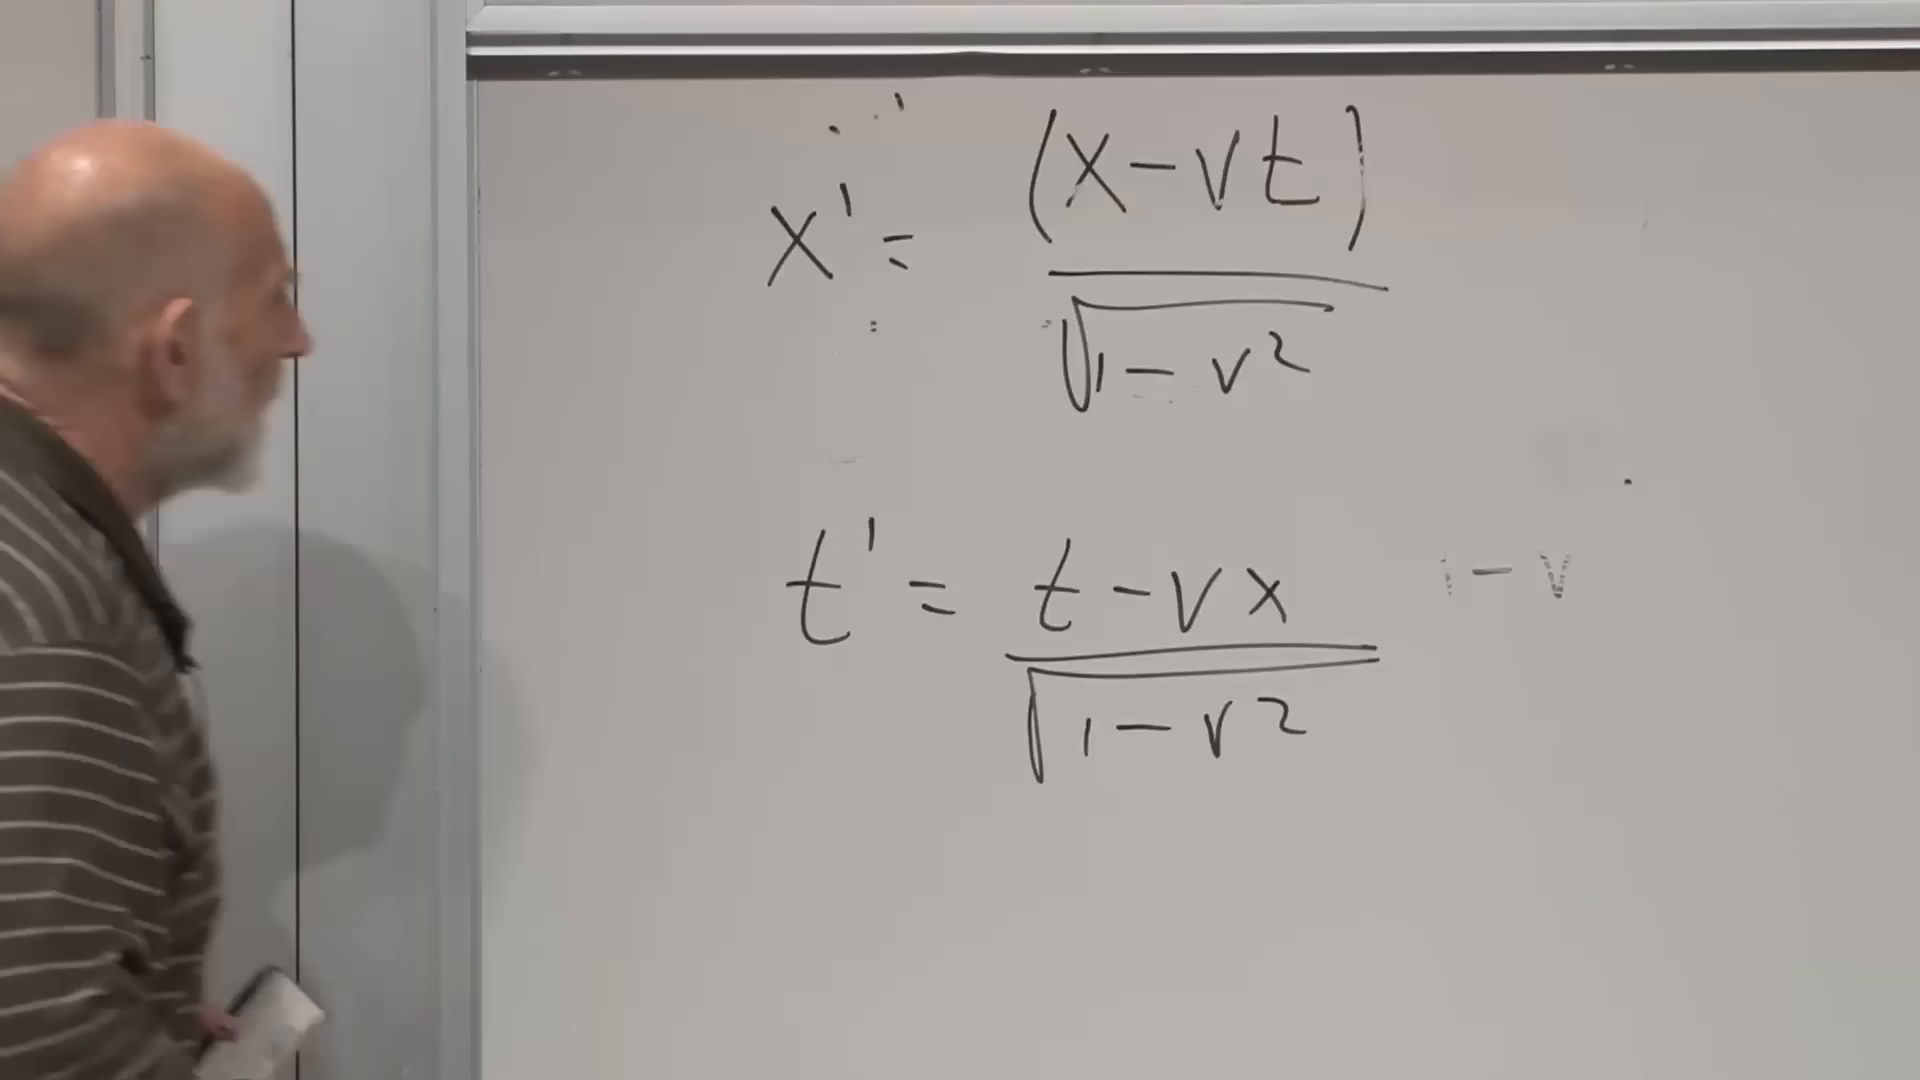
\includegraphics[width=0.90\textwidth]{lecture_01_figure_08.png}
\caption{光速が1である単位での、完成したローレンツ変換。}
\lectureframe{01:02:05}
\end{figure}

\subsection{通常の単位の復元}

次元解析により通常の単位が復元される。分母は無次元比\(v^2/c^2\)のみに依存しうる一方、時間の式における\(vx\)は\(vx/c^2\)にならなければならない：
\begin{align}
x'&=\gamma(x-vt),&
t'&=\gamma\left(t-\frac{vx}{c^2}\right),
\label{eq:sr1-lorentz-dimensional}\\
\gamma&=\frac{1}{\sqrt{1-v^2/c^2}}.
\label{eq:sr1-gamma}
\end{align}
逆変換は
\begin{align}
x&=\gamma(x'+vt'),&
t&=\gamma\left(t'+\frac{vx'}{c^2}\right).
\label{eq:sr1-lorentz-inverse-dimensional}
\end{align}

\begin{figure}[htbp]
\centering
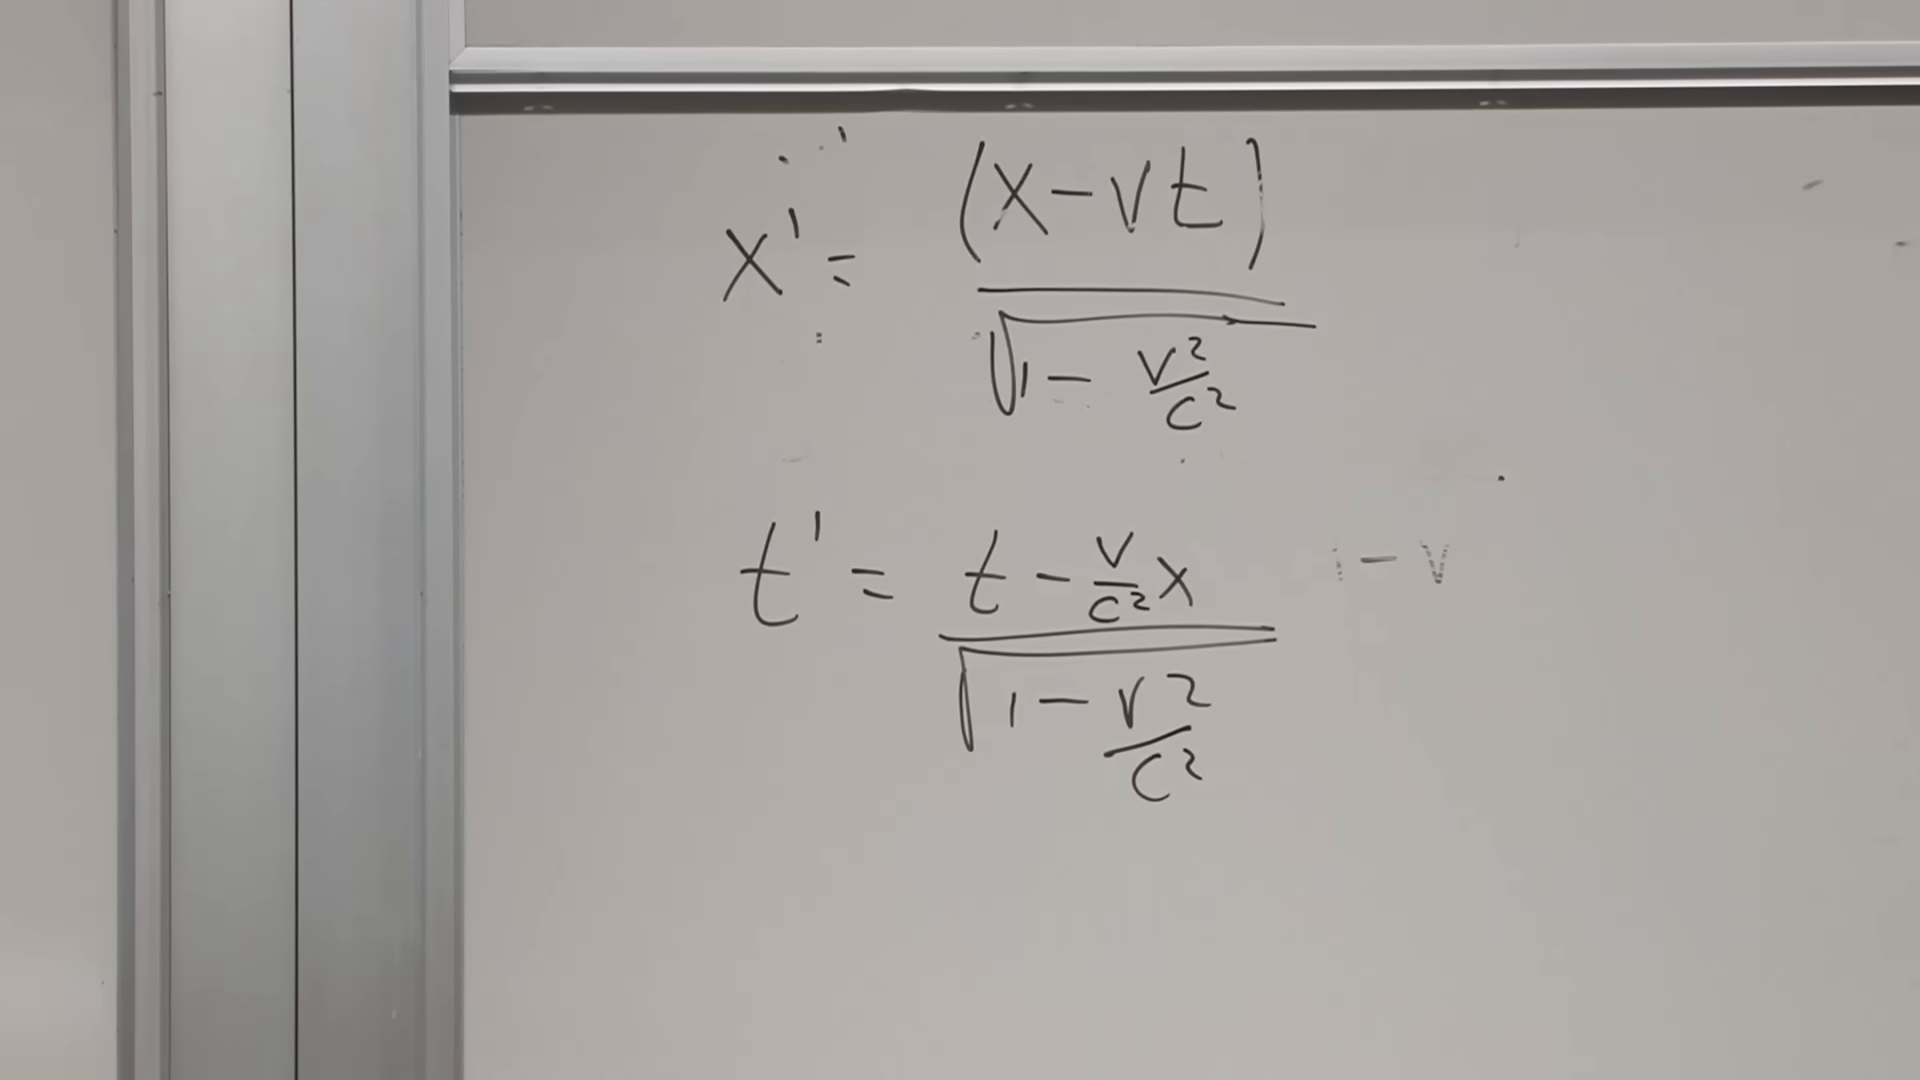
\includegraphics[width=0.90\textwidth]{lecture_01_figure_09.png}
\caption{\(c\)を復元したローレンツの式：\(v^2/c^2\)がスケールを支配し、\(vx/c^2\)が位置を時間に混ぜる。}
\lectureframe{01:05:01}
\end{figure}

\(v\ll c\)のとき、
\begin{equation}
\gamma=1+\frac{1}{2}\frac{v^2}{c^2}+O\!\left(\frac{v^4}{c^4}\right),
\end{equation}
であり、変換は
\begin{equation}
x'\approx x-vt,
\qquad
t'\approx t.
\end{equation}
に帰着する。地球上の速度では比は通常ごく小さく、これがニュートン運動学の成功を説明する。\(c\)の近くでは、補正は大きくなる。

運動は\(x\)軸に沿って選ばれた。横方向の測定腕は、相反性を破ることなく一方の慣性系を他方から区別することはできないので、
\begin{equation}
y'=y,
\qquad
z'=z.
\end{equation}

\section{運動する棒の測定}

長さとは、測定を行う系で同時に測られた両端点の間隔を意味する。写真に撮られた物体の見かけの角的大きさを意味するのではない。光の伝播遅延が別個の光学的问题を持ち込むからである。

棒がプライムなし系で静止しており、端点が
\begin{equation}
x=0,
\qquad
x=1.
\end{equation}
であるとする。プライム系の観測者は、単一のプライム系同時刻面、たとえば\(t'=0\)上で端点事象を測定する。遠い方の端点\(x=1\)では、
\begin{equation}
t'=0
\quad\Longrightarrow\quad
t=\frac{vx}{c^2}.
\end{equation}
一時的に\(c=1\)に戻ると、この事象は\(t=v\)を持ち、
\begin{equation}
x'=\frac{x-vt}{\sqrt{1-v^2}}
   =\frac{1-v^2}{\sqrt{1-v^2}}
   =\sqrt{1-v^2}.
\end{equation}

\begin{figure}[htbp]
\centering
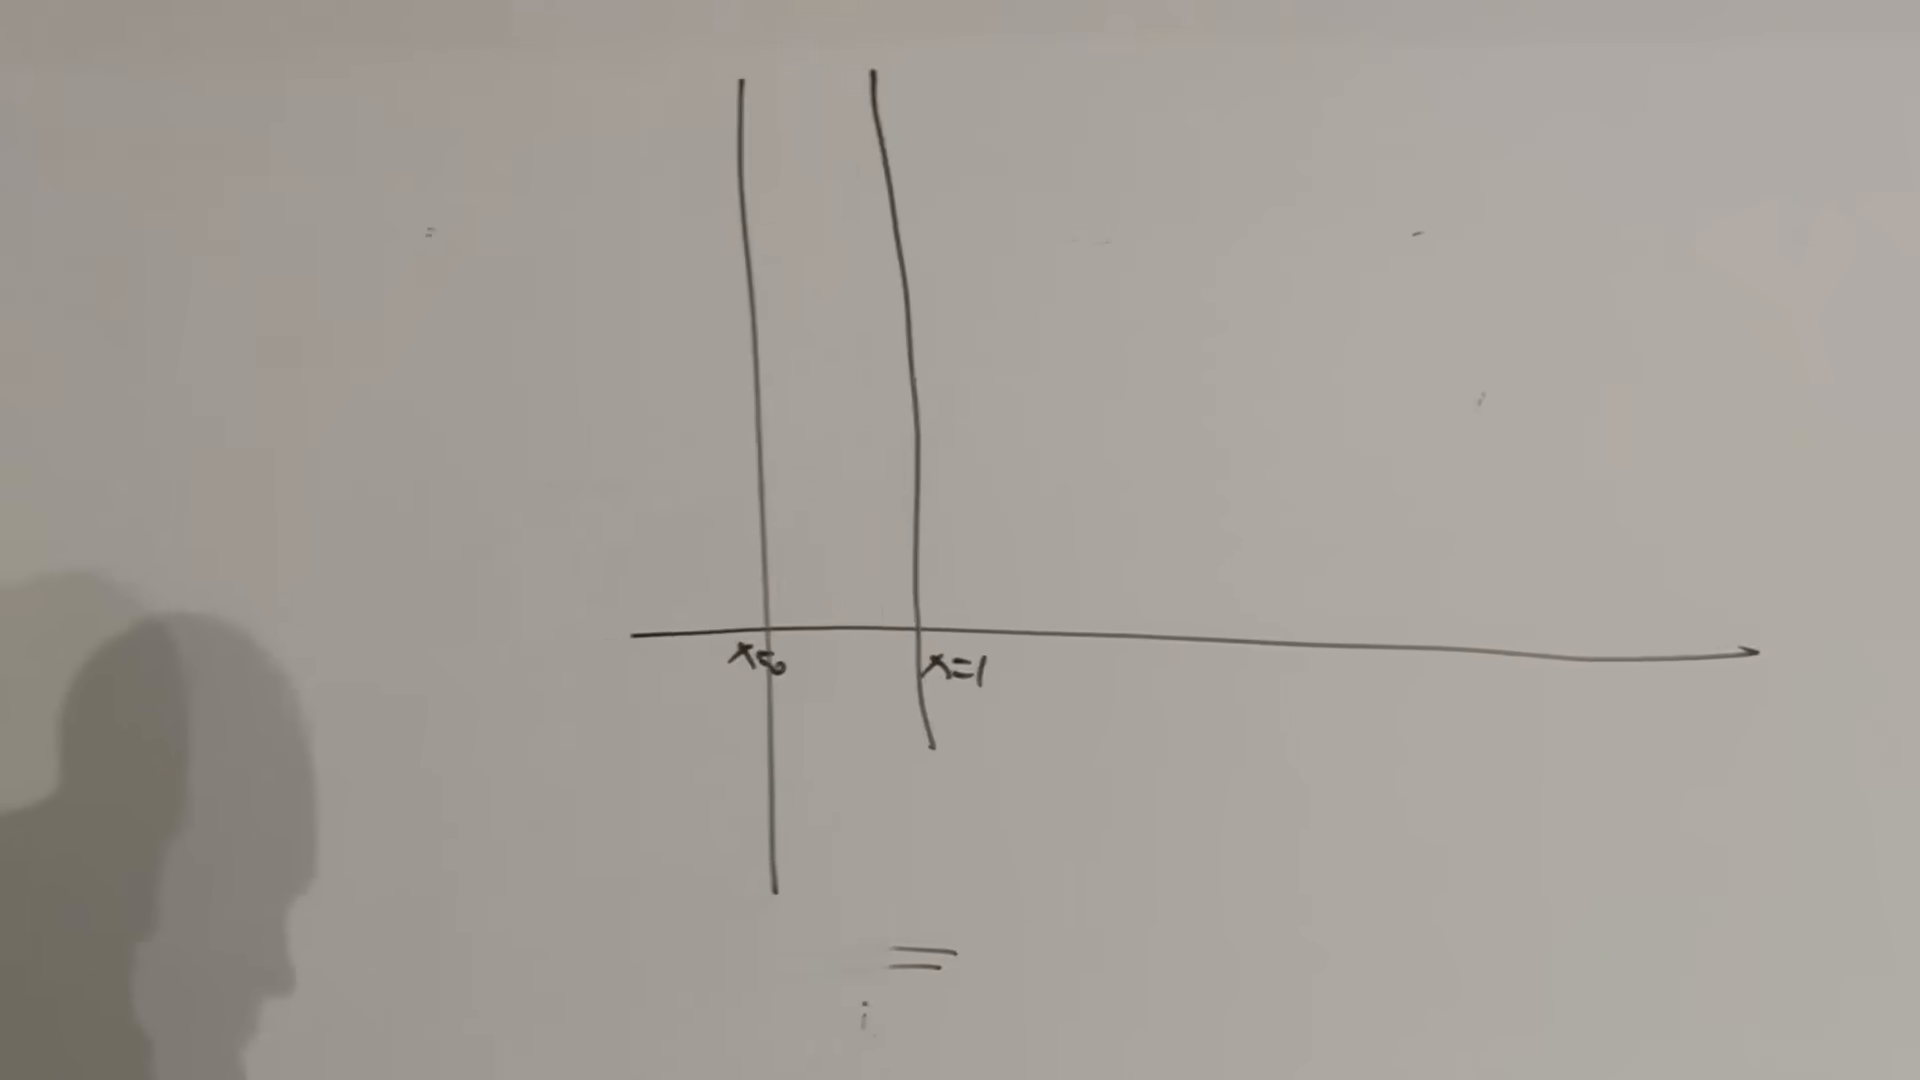
\includegraphics[width=0.90\textwidth]{lecture_01_figure_10.png}
\caption{プライムなし系で静止している棒の世界線\(x=0\)と\(x=1\)；運動する観測者はそれらを一つの\(t'\)面で比較しなければならない。}
\lectureframe{01:11:14}
\end{figure}

\begin{figure}[htbp]
\centering
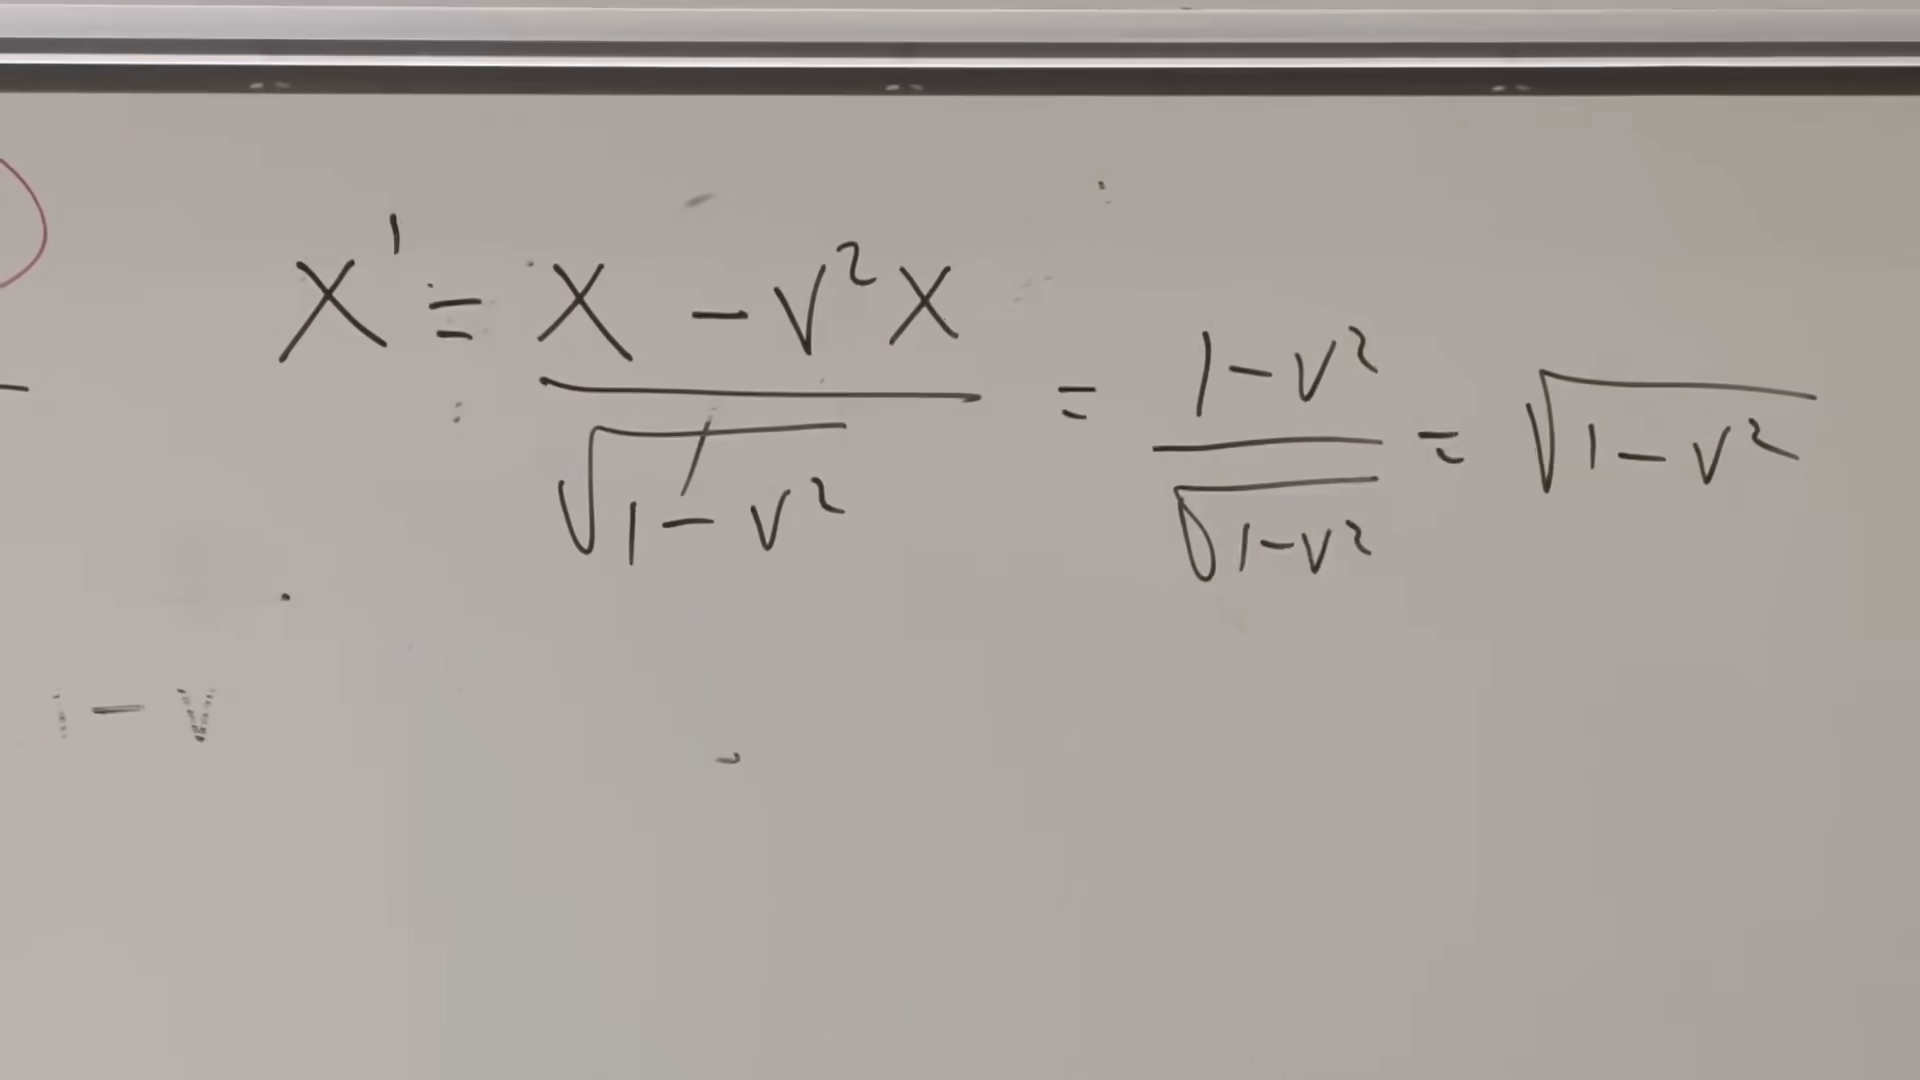
\includegraphics[width=0.90\textwidth]{lecture_01_figure_11.png}
\caption{プライム系での同時端点測定は、単位\(c=1\)で収縮因子\(\sqrt{1-v^2}\)を与える。}
\lectureframe{01:16:03}
\end{figure}

単位を復元し、一般的な静止長\(L_0\)を用いると、
\begin{equation}
L=\frac{L_0}{\gamma}
 =L_0\sqrt{1-\frac{v^2}{c^2}}.
\label{eq:sr1-length-contraction}
\end{equation}

\begin{classroomqa}
\audiencequestion{棒の遠い端が\(x=1\)にあるなら、その座標も\(x'=1\)であるべきではないか？}
\lecturerresponse{そうではない。棒はプライムなし系で静止しているので、\(x=0\)と\(x=1\)はそこでの固定された端点を表す。遠い端点のプライム系座標は時間とともに変化する。測定面\(t'=0\)上でのその値こそ、ローレンツ変換が計算するものである。\lecturetimestamp{01:14:24}}
\end{classroomqa}

\begin{classroomqa}
\audiencequestion{各慣性観測者が、他方の観測者の棒の方が短いと矛盾なく言えるのはなぜか？}
\lecturerresponse{彼らは異なる端点事象の対を測定している。プライムなし系の観測者は\(t\)が等しいことを要求し、プライム系の観測者は\(t'\)が等しいことを要求する。同時性は系に依存するので、それら二つの端点対は同じ事象の対ではない。したがって相反性は矛盾を生じない。\lecturetimestamp{01:16:28}}
\end{classroomqa}

操作的版を明示しておく価値がある。測定系に沿って同期した時計と助手を配置する。定められた現地時刻に、各助手は近くを通過する端点の位置を記録する。同時に記録されたそれら二つの位置の差が、その系における棒の長さを与える。棒がたまたまどう見えるかには何も依存しない。

\begin{classroomqa}
\audiencequestion{\(c=1\)のとき、単位棒は1光秒の長さでなければならないのだろうか。}
\lecturerresponse{時間を秒で測る場合に限られる。代わりに長さにはメートルを用い、時間は1メートルを光が進む時間で測ってもよい。\(c=1\)と置くことは時間と長さの単位を結び付けるが、どちらの物理単位を先に選ぶべきかは規定しない。\lecturetimestamp{01:21:17}}
\end{classroomqa}

\section{運動する時計と双子の問い}

次に、プライム系で静止している時計を追う。その世界線に沿って、
\begin{equation}
x'=0.
\end{equation}
この時計が\(t'=1\)を指す事象と原点を比較する。逆変換により
\begin{equation}
t=\gamma\left(t'+\frac{vx'}{c^2}\right)=\gamma.
\end{equation}
が得られる。したがって、運動する時計の経過時間1単位は、プライムなし座標時間の\(\gamma\)単位に対応する：
\begin{equation}
\Delta t=\gamma\,\Delta\tau,
\qquad
\Delta\tau=\frac{\Delta t}{\gamma}.
\label{eq:sr1-time-dilation}
\end{equation}

\begin{figure}[htbp]
\centering
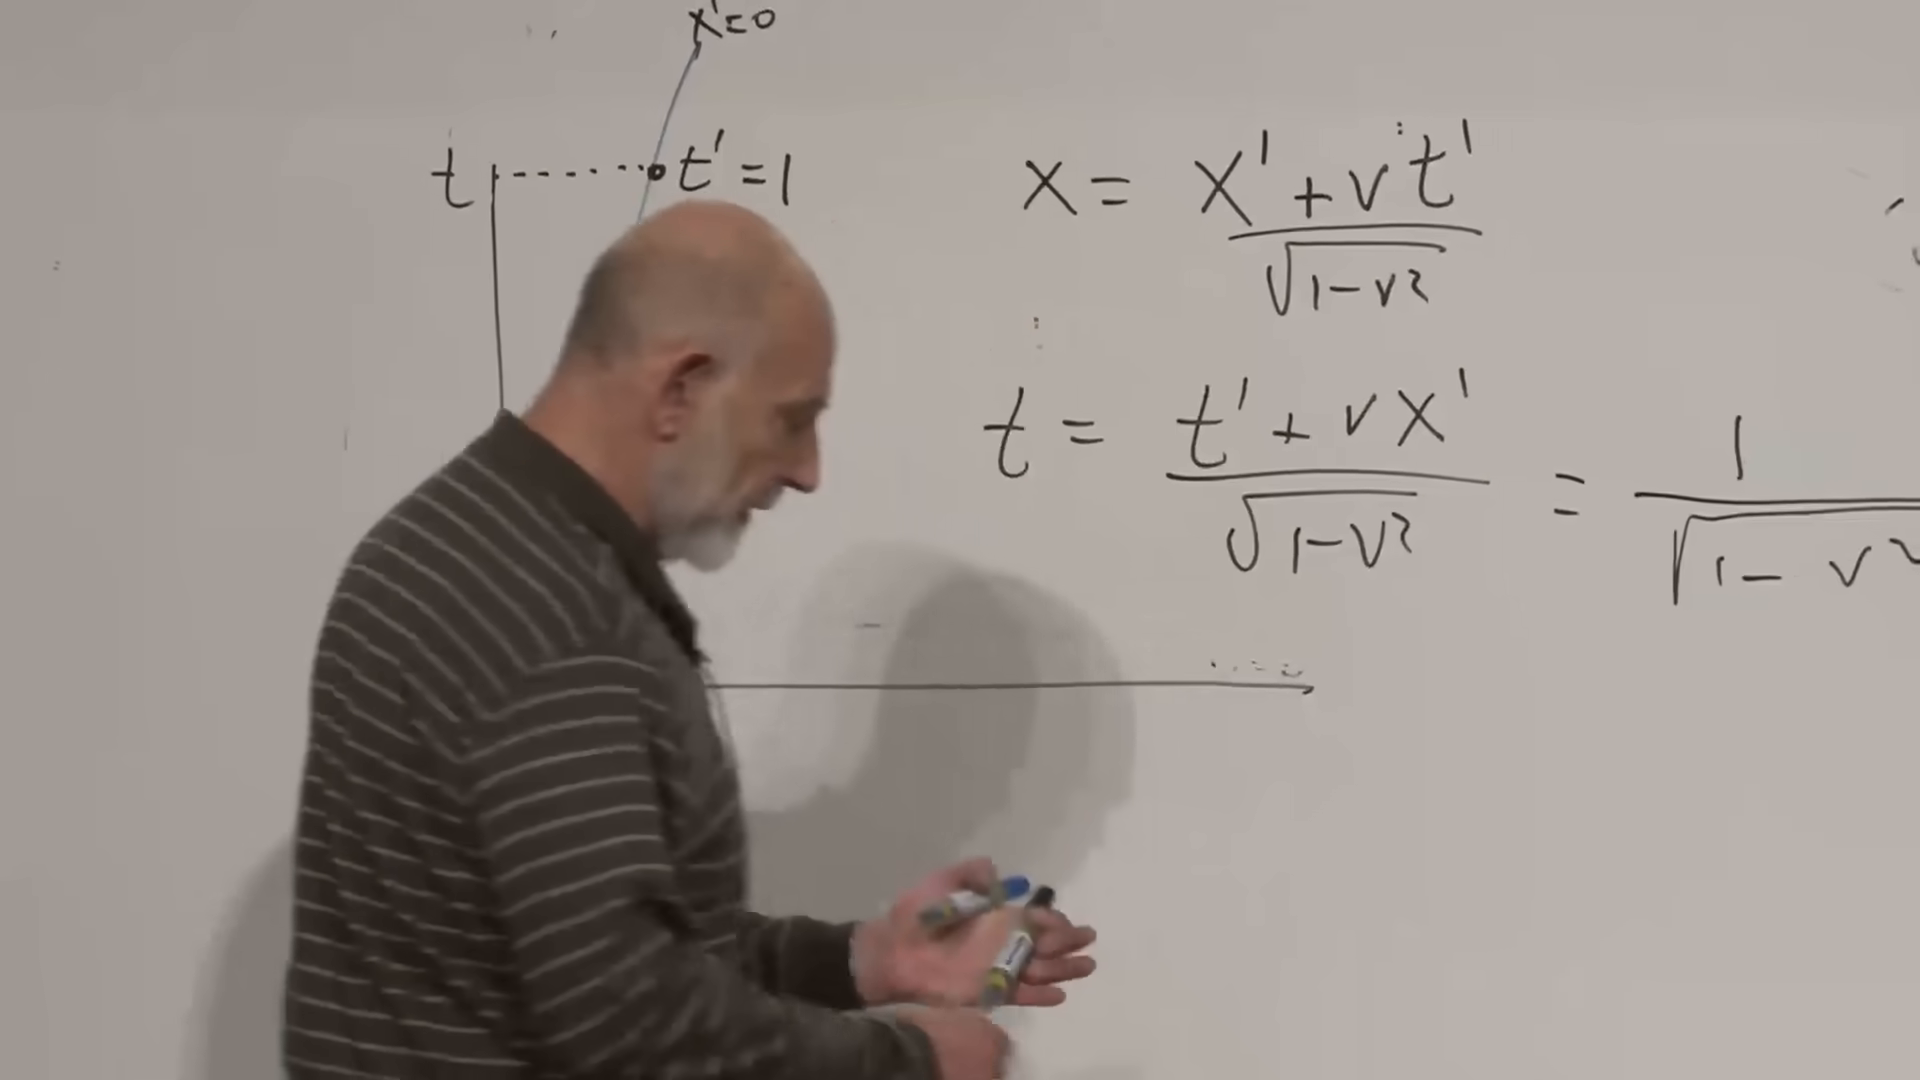
\includegraphics[width=0.90\textwidth]{lecture_01_figure_12.png}
\caption{\(x'=0\)上で運ばれる時計は、同じ2つの事象の間で、静止座標時間よりも少ない経過時間を記録する：\(t=\gamma t'\)。}
\lectureframe{01:26:42}
\end{figure}

この効果は、時計と呼ばれる仕組みだけではなく、あらゆる物理的な時計に関わる。腕時計、原子遷移、代謝、生物学的老化はすべて同じ固有時従う。ニューヨークの路上で買った安物の時計は、粗悪なロレックスであることによって相対性理論を免れることはない。不正確な時を刻むかもしれないが、それが用いる過程はどのようなものであれ、同じ運動学に従う。

\begin{classroomqa}
\audiencequestion{各慣性観測者が相手の時計が遅れて進むと見るなら、なぜ旅行する双子の方が若く帰ってくるのか。}
\lecturerresponse{往復は、大域的に等価な2つの慣性世界線の比較ではない。旅行者は向きを変えて別の慣性系に移らなければならないが、家に残る双子は1つの慣性世界線上にとどまる。向きを変えることが交換対称性を破るため、蓄積された固有時は異なりうる。\lecturetimestamp{01:26:37}}
\end{classroomqa}

\begin{classroomqa}
\audiencequestion{年齢差を引き起こすのは、向きを変える間の加速度そのものなのか。}
\lecturerresponse{加速度は対称性が破れる場所を示すが、年齢差は完全な経路に沿って固有時を積分することによって計算される。向きを変える期間は短くしてもよく、また慣性区間間の移行として扱ってもよい。等しくない時空経路は依然として等しくない固有時をもつ。\lecturetimestamp{01:29:20}}
\end{classroomqa}

\section{不変な幾何学}

時間の遅れの図は、ユークリッド幾何学で読むと異常に見える。斜めの経路は斜辺のように見えるのに、垂直な経路よりも少ない固有時を運ぶ。解決は代数のごまかしではない。時空は異なる計量をもつのである。

ユークリッド平面では、回転は\(x\)と\(y\)を変えるが、
\begin{equation}
x'^2+y'^2=x^2+y^2.
\label{eq:sr1-euclidean-invariant}
\end{equation}
を保つ。ローレンツ変換が\(t^2+x^2\)を保つかどうかを試すのは自然である。それは保たない。単位\(c=1\)では、
\begin{align}
t'^2
&=\frac{t^2-2vtx+v^2x^2}{1-v^2},\\
x'^2
&=\frac{x^2-2vtx+v^2t^2}{1-v^2}.
\end{align}
加えると係数が誤ってしまう。代わりに引くと混合項が相殺され、
\begin{align}
t'^2-x'^2
&=
\frac{t^2-2vtx+v^2x^2-x^2+2vtx-v^2t^2}{1-v^2}\\
&=t^2-x^2.
\label{eq:sr1-interval-invariance}
\end{align}
が得られる。

\begin{figure}[htbp]
\centering
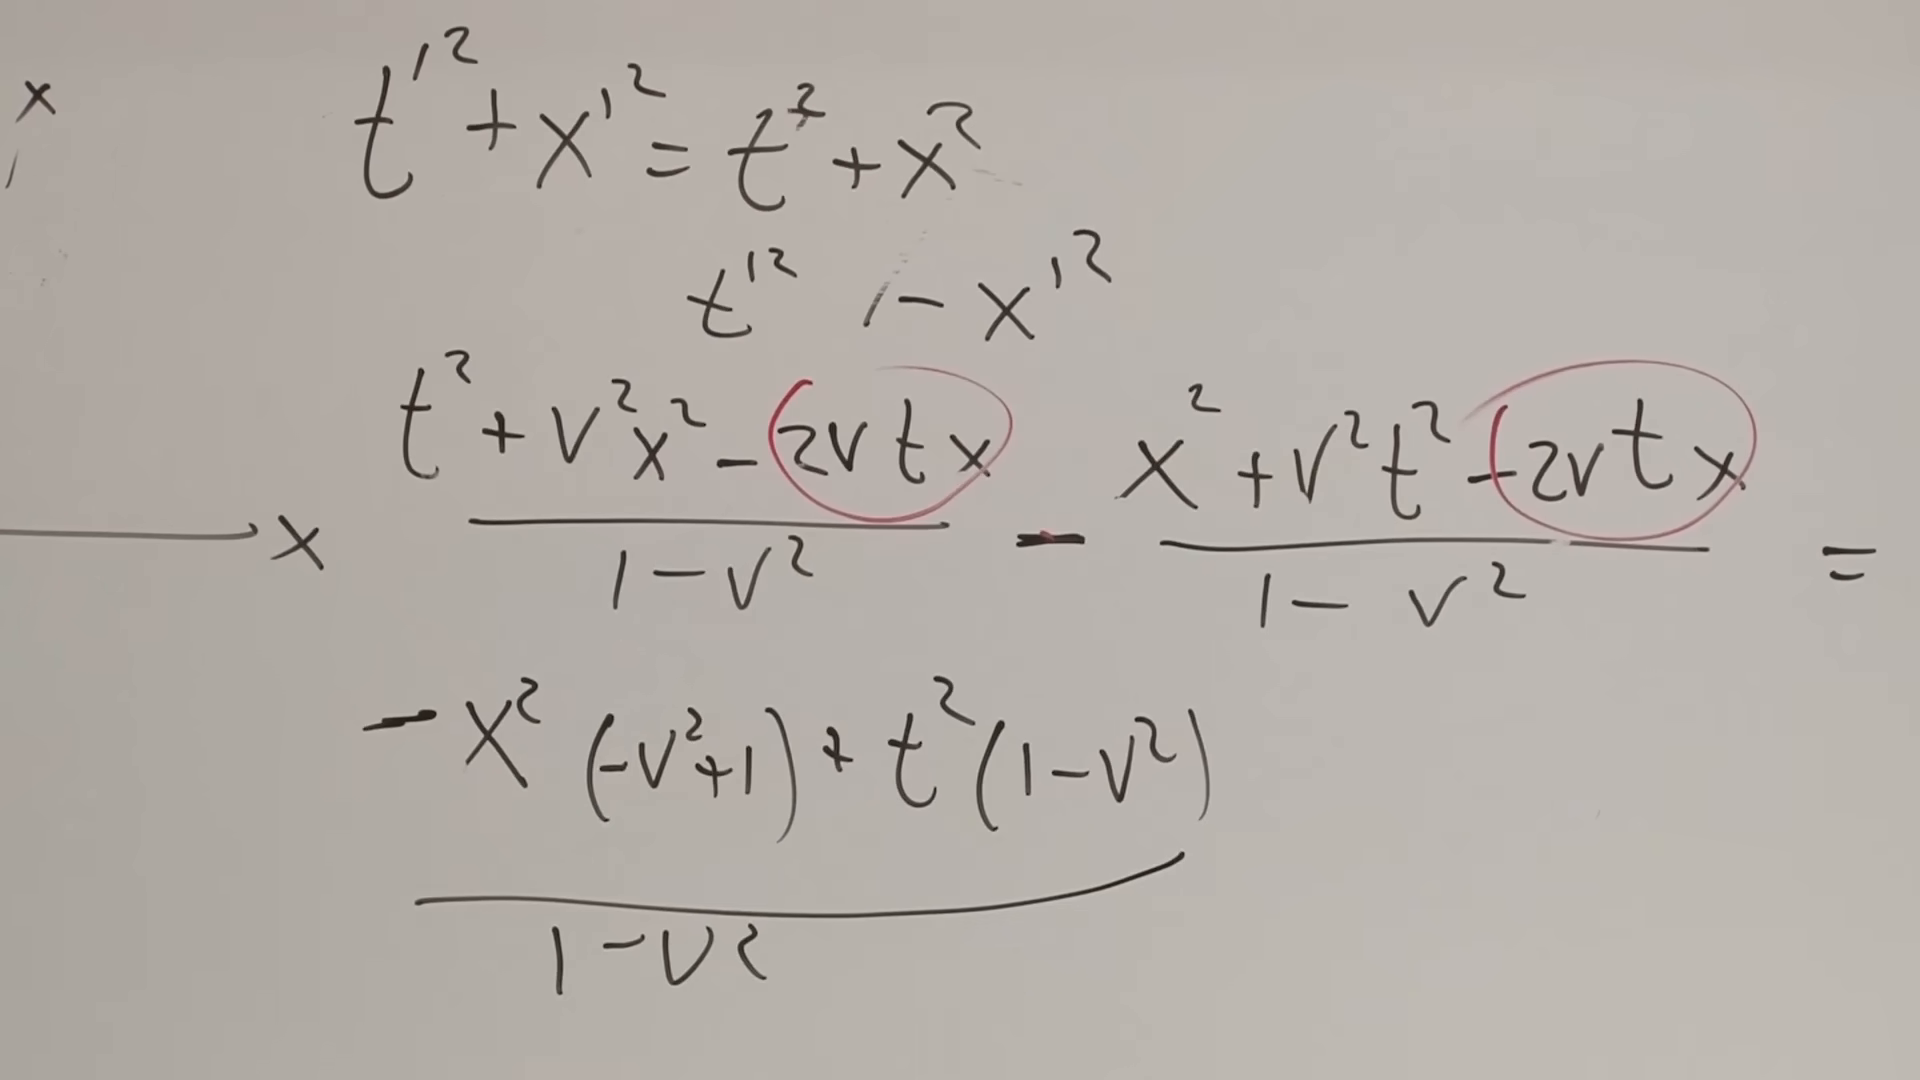
\includegraphics[width=0.90\textwidth]{lecture_01_figure_13.png}
\caption{変換後の座標の二乗を引くと交差項が相殺され、不変量\(t^2-x^2\)が現れる。}
\lectureframe{01:38:07}
\end{figure}

座標は系に依存する成分である。組み合わせ
\begin{equation}
\Delta s^2=c^2\Delta t^2-\Delta x^2
\label{eq:sr1-spacetime-interval}
\end{equation}
はすべての慣性系で同じである。空間次元が増えると、
\begin{equation}
\Delta s^2
=c^2\Delta t^2-\Delta x^2-\Delta y^2-\Delta z^2.
\end{equation}

\begin{classroomqa}
\audiencequestion{斜辺の方が長いという通常の幾何学の規則を捨てることは、なぜ正当化されるのか。}
\lecturerresponse{その規則は正定値ユークリッド計量に属する。ここでの座標は棒、時計、光信号によって操作的に定義され、その変換は二乗の差を保つ。ミンコフスキー幾何学は逆説を回避するために仮定されるのではなく、それらの測定から発見されるのである。\lecturetimestamp{01:43:21}}
\end{classroomqa}

\subsection{固有時}

時計の世界線上にある2つの事象について、その時計の静止系を選ぶ。そこでは\(\Delta x'=0\)であるから、不変性により
\begin{equation}
c^2\Delta\tau^2
=c^2\Delta t^2-\Delta x^2,
\end{equation}
または
\begin{equation}
\Delta\tau
=\sqrt{\Delta t^2-\frac{\Delta x^2}{c^2}}.
\label{eq:sr1-proper-time}
\end{equation}
が得られる。これは2つの事象の間でその時計が記録する実際の時間である。

\begin{figure}[htbp]
\centering
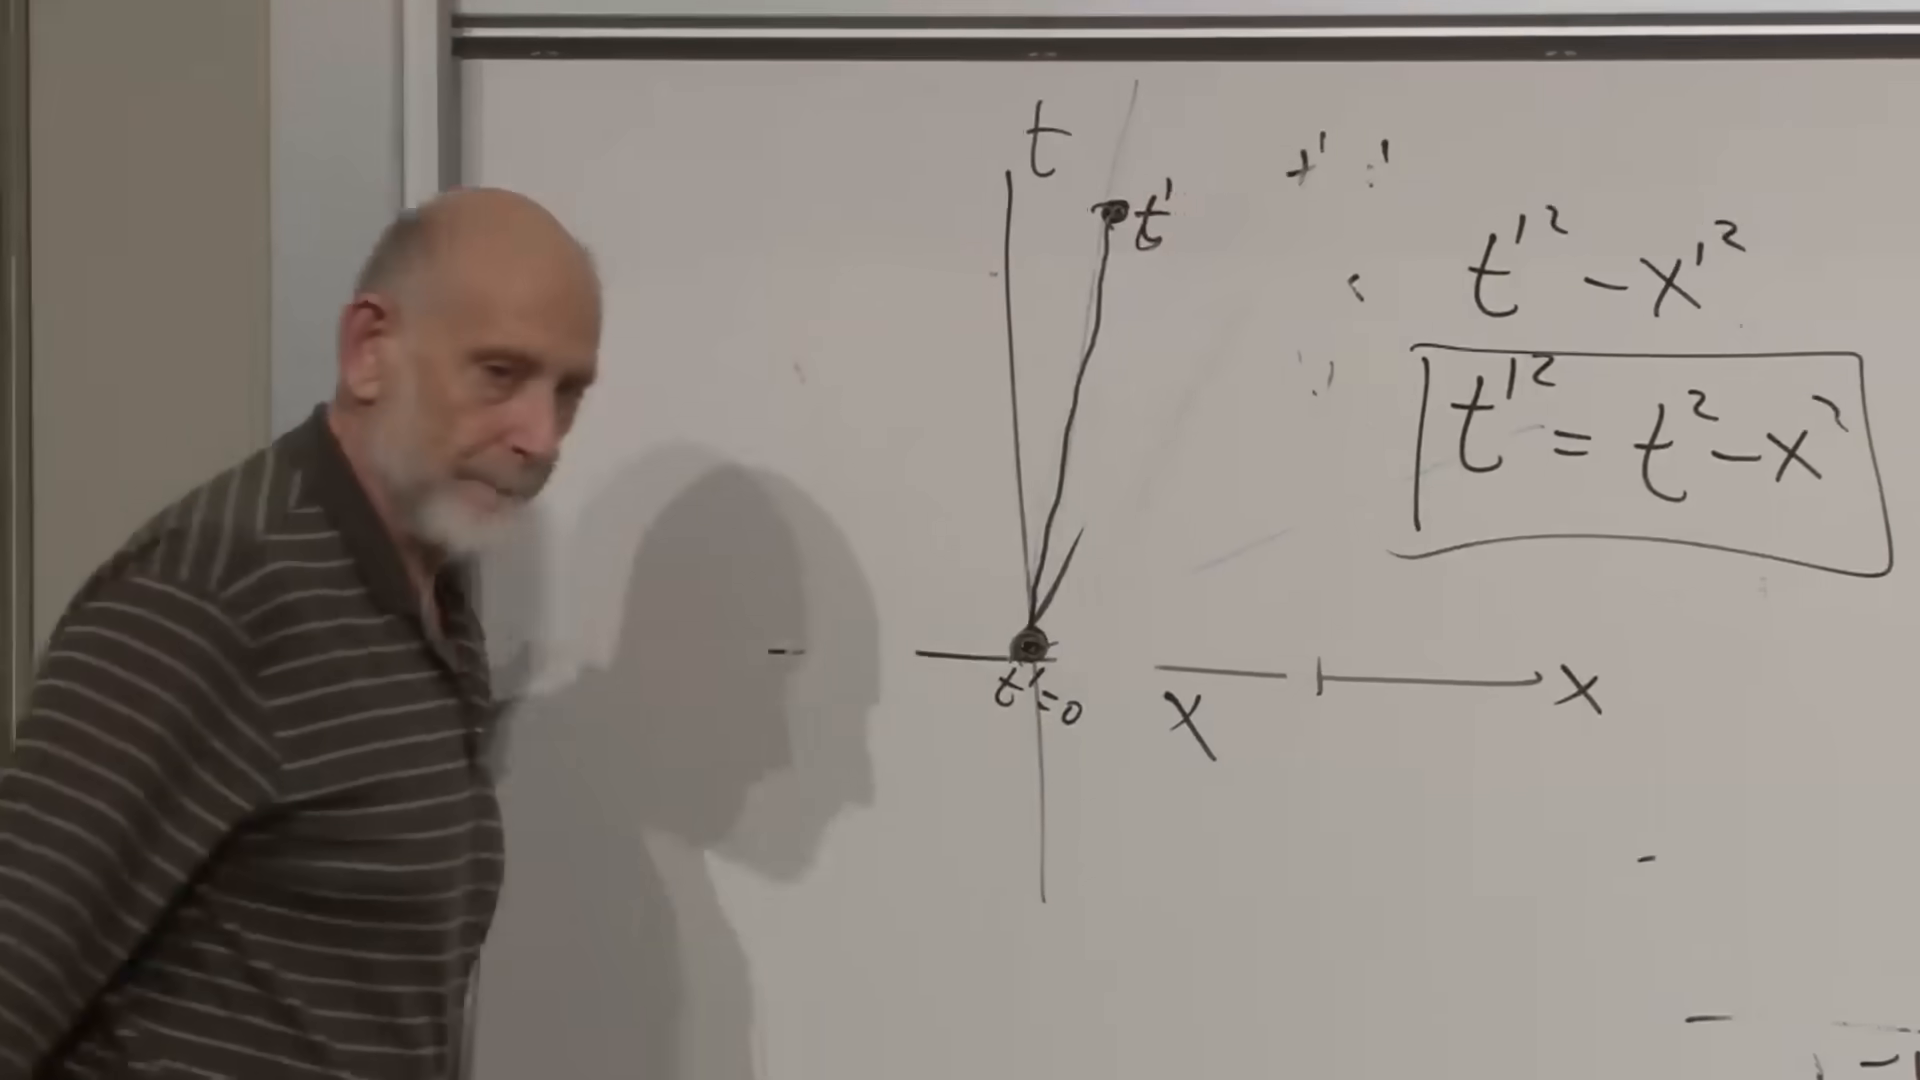
\includegraphics[width=0.90\textwidth]{lecture_01_figure_14.png}
\caption{時計の静止系では空間的隔たりが消えるため、不変間隔はその固有時の二乗になる。}
\lectureframe{01:41:28}
\end{figure}

\begin{classroomqa}
\audiencequestion{固有時は\(t^2-x^2/c^2\)なのか、それともその平方根なのか。}
\lecturerresponse{二乗の差は固有時の二乗である。共通の原点から測った隔たりに対して、時計が読み取る経過時間は\(\tau=\sqrt{t^2-x^2/c^2}\)である。当初の表現で欠けていた平方根を復元しなければならない。\lecturetimestamp{01:51:02}}
\end{classroomqa}

\subsection{時間的、光的、空間的隔たり}

2つの異なる事象は間隔がゼロでありうる。単位\(c=1\)では、
\begin{equation}
\Delta t^2-\Delta x^2=0
\quad\Longleftrightarrow\quad
\Delta x=\pm\Delta t.
\end{equation}
そのような事象は光線によって結ばれている。

\begin{figure}[htbp]
\centering
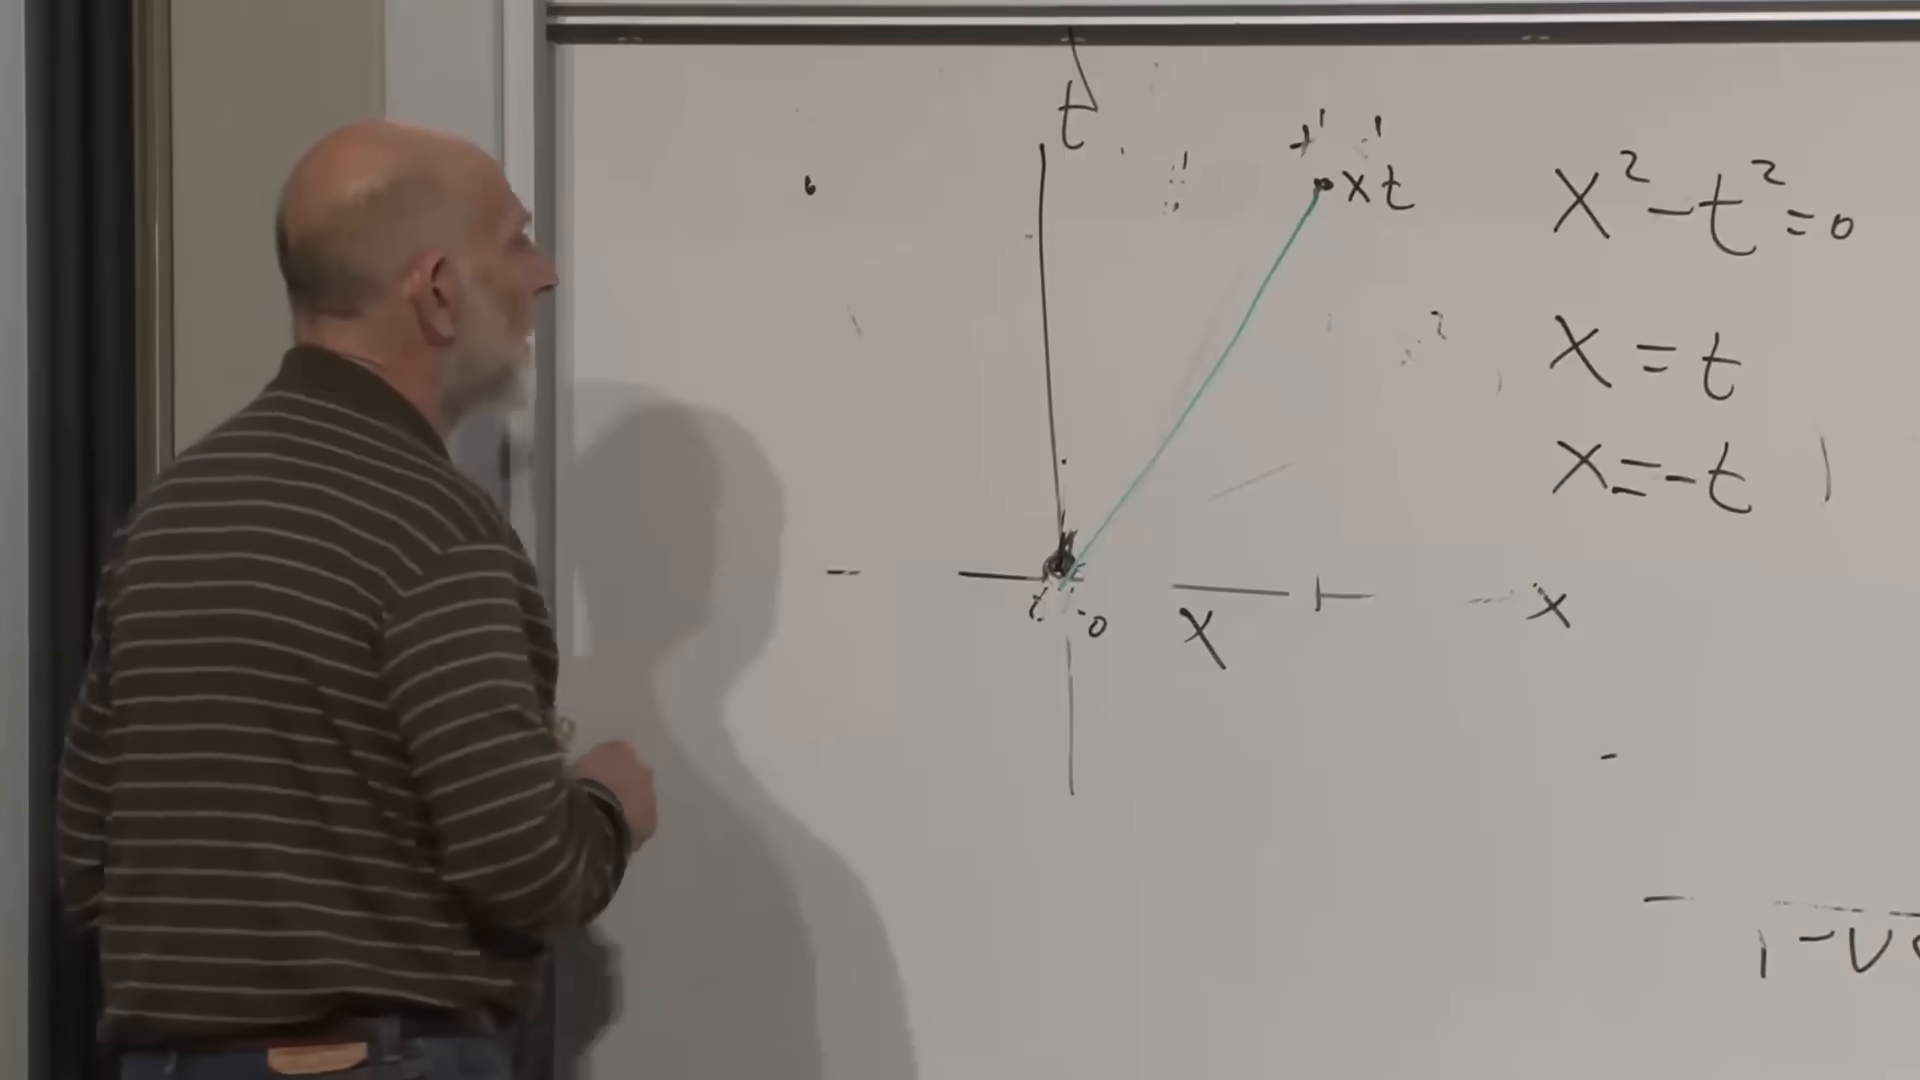
\includegraphics[width=0.90\textwidth]{lecture_01_figure_15.png}
\caption{ヌル分離した事象は\(x=\pm t\)上にあり、そこでは時空間隔と光速経路の固有時間がゼロになる。}
\lectureframe{01:46:40}
\end{figure}

もし光が通常の時計を運べるとしたら、放出から吸収までの間に固有時間の刻みは生じない。これは光にとって有効な静止系ではなく、すべてのヌル線分がゼロの固有時間をもつという極限的な主張である。

光線は時空を三つの不変なクラスに分ける：
\begin{align}
c^2\Delta t^2-\Delta x^2&>0
&&\text{timelike},\\
c^2\Delta t^2-\Delta x^2&=0
&&\text{null},\\
c^2\Delta t^2-\Delta x^2&<0
&&\text{spacelike}.
\end{align}
物理的な時計は時間的隔たりをもつ事象を結ぶことができ、正の間隔がその固有時間を定める。亜光速の物体は空間的隔たりをもつ事象を結ぶことはできない。空間的な対に対しては、事象が同時となる系を選び、固有距離を定義することができる
\begin{equation}
\ell_{\rm proper}
=\sqrt{\Delta x^2-c^2\Delta t^2}.
\end{equation}

\begin{figure}[htbp]
\centering
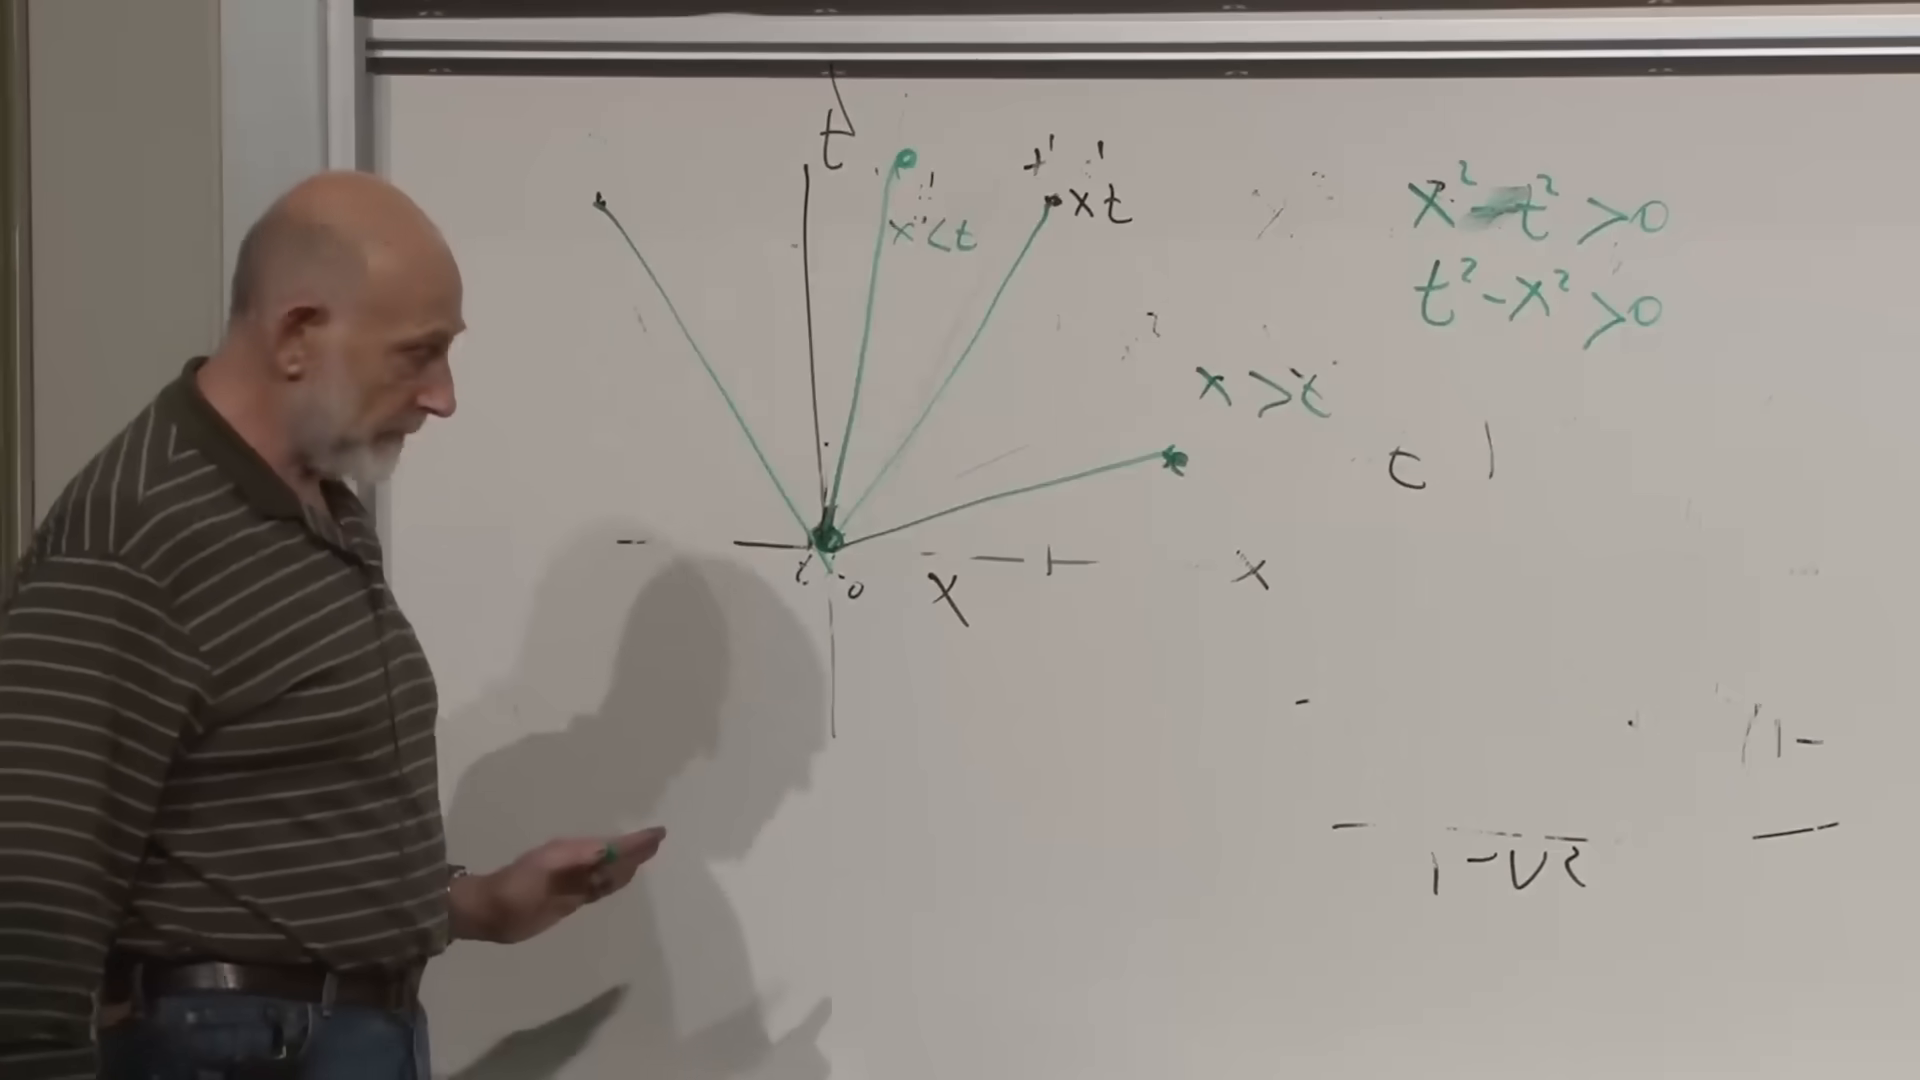
\includegraphics[width=0.90\textwidth]{lecture_01_figure_16.png}
\caption{光円錐は、時計が結ぶことのできる時間的対と、亜光速の物体が結ぶことのできない空間的対とを分ける。}
\lectureframe{01:48:47}
\end{figure}

\begin{classroomqa}
\audiencequestion{不変量はいつ固有時間と呼ばれるべきで、いつ固有長と呼ばれるべきか？}
\lecturerresponse{時間的対に対しては、両方の事象が一つの場所で起こる静止系が存在し、間隔が固有時間を与える。空間的対に対しては、両方が一つの時刻に起こる系が存在し、逆符号の不変量がそれらの固有距離を与える。ヌル分離は両者の境界である。 \lecturetimestamp{01:47:22}}
\end{classroomqa}

\begin{classroomqa}
\audiencequestion{単位が\(c=1\)となるように選ばれていないとき、\(c\)はどこに属するのか？}
\lecturerresponse{不変量は\(c^2\Delta t^2-\Delta x^2\)であり、長さの二乗の次元をもつ。\(c^2\)で割ると\(\Delta\tau^2=\Delta t^2-\Delta x^2/c^2\)となり、時間の二乗の次元をもつ。 \lecturetimestamp{01:49:56}}
\end{classroomqa}

\section{ローレンツ対称性とその歴史的意味}

\begin{classroomqa}
\audiencequestion{ローレンツ変換は回転とみなせるか？}
\lecturerresponse{はい、ただし通常のユークリッド回転としてではない。それは\(t^2-x^2\)を保存する双曲的回転である。歴史的には虚角による回転として記述できるが、ラピディティが現代的な実パラメータ表示を与える。 \lecturetimestamp{01:51:40}}
\end{classroomqa}

アインシュタインの道筋は電磁気学と密接に結びついていた。彼の後の回想によれば、すでに十代の頃、光波を追いかけたら何が起こるかを考えていた。ガリレイ的な速度の引き算では波は静止して見えるはずだが、マクスウェル方程式には真空中に対応する凍結した振動光波は存在しない。この矛盾は、測定棒の特異な力学的性質ではなく、運動学を指し示していた。

\begin{classroomqa}
\audiencequestion{アインシュタインの議論は主にマイケルソン--モーリーのような実験への応答だったのか？}
\lecturerresponse{実験的背景は歴史的に重要だったが、アインシュタイン自身の証言はマクスウェル方程式の構造と光線を追いかける思考実験を強調していた。彼が特定の干渉計の結果をどれほど知っていたか、あるいはそれに依拠していたかは歴史的に議論されており、明確な物理的要点はマクスウェル変換とガリレイ変換の間の対称性の矛盾である。 \lecturetimestamp{01:52:04}}
\end{classroomqa}

マクスウェル方程式はガリレイ変換ではなくローレンツ変換の下で不変である。ローレンツとフィッツジェラルドはすでに、エーテルを保持し、収縮をエーテル中を運動することによって引き起こされる力学的変形と解釈しながら、関連する収縮の式を見出していた。その見方では、この効果はさらなる補正を伴う近似的な物質応答でありえたかもしれない。

アインシュタインの決定的な一歩は、相対性原理と不変な光速度を厳密な運動学の原理とすることだった。すると長さの収縮と時間の遅れは、エーテルが及ぼす特別な力ではなく、慣性系を関係づける幾何学を表すため、あらゆる適切な棒と時計に適用される。次の課題は、この幾何学の内部で粒子の運動を定式化することである。
